%=============================================================================
%  INFORME DE INVESTIGACIÓN DE MERCADO
%  Demanda Global de Servicios de Consultoría e Ingeniería en la Gran Minería
%  Horizonte 2030
%  Preparado para: Comité de Estrategia — REDCO Mining Consultants
%  Motor de compilación: pdflatex (3 pasadas para TOC / referencias)
%  Todos los gráficos están construidos con TikZ / pgfplots.
%=============================================================================
\documentclass[11pt,letterpaper]{report}

% ---- Idioma y codificación -------------------------------------------------
\usepackage[utf8]{inputenc}
\usepackage[T1]{fontenc}
\usepackage[main=spanish,provide=*]{babel}
\usepackage{lmodern}

% ---- Geometría y espaciado -------------------------------------------------
\usepackage[margin=1in,headheight=14pt]{geometry}
\usepackage{setspace}
\usepackage{parskip}
\usepackage{ragged2e}

% ---- Color -----------------------------------------------------------------
\usepackage{xcolor}
\definecolor{primaryblue}{RGB}{0,51,102}     % navy corporativo
\definecolor{accentblue}{RGB}{0,114,178}     % Okabe-Ito azul
\definecolor{accentgreen}{RGB}{0,158,115}    % verde
\definecolor{accentorange}{RGB}{230,159,0}   % naranja
\definecolor{accentred}{RGB}{213,94,0}       % bermellón
\definecolor{accentsky}{RGB}{86,180,233}     % celeste
\definecolor{accentpurple}{RGB}{204,121,167} % magenta
\definecolor{lightgray}{RGB}{238,238,238}
\definecolor{tablealt}{RGB}{234,240,247}
\definecolor{tablehead}{RGB}{0,51,102}
\definecolor{darkgray}{RGB}{90,90,90}
\definecolor{riskhi}{RGB}{200,60,40}
\definecolor{riskmed}{RGB}{235,170,40}
\definecolor{risklo}{RGB}{90,170,90}

% ---- Gráficos y TikZ -------------------------------------------------------
\usepackage{graphicx}
\usepackage{tikz}
\usepackage{pgfplots}
\pgfplotsset{compat=1.16}
\usepgfplotslibrary{fillbetween}
\usetikzlibrary{positioning,shapes.geometric,shapes.misc,arrows.meta,calc,fit,backgrounds,patterns}

% ---- Tablas ----------------------------------------------------------------
\usepackage{longtable}
\usepackage{booktabs}
\usepackage{array}
\usepackage{multirow}
\usepackage{colortbl}
\usepackage{tabularx}

% ---- Cajas / destacados ----------------------------------------------------
\usepackage[most]{tcolorbox}

% ---- Matemática ------------------------------------------------------------
\usepackage{amsmath}
\usepackage{amssymb}

% ---- Listas ----------------------------------------------------------------
\usepackage{enumitem}
\setlist{nosep,leftmargin=1.4em}

% ---- Encabezados y pie -----------------------------------------------------
\usepackage{fancyhdr}
\usepackage{titlesec}

% ---- Pies de figura/tabla --------------------------------------------------
\usepackage{caption}
\captionsetup{font=small,labelfont=bf,labelsep=period}

% ---- Hiperenlaces (último) -------------------------------------------------
\usepackage[hidelinks]{hyperref}

%=============================================================================
%  ESTILO DE TÍTULOS
%=============================================================================
\titleformat{\chapter}[hang]
  {\normalfont\Huge\bfseries\color{primaryblue}}
  {\thechapter\hspace{12pt}\textcolor{accentorange}{\rule[2pt]{2pt}{22pt}}\hspace{12pt}}{0pt}{}
\titlespacing*{\chapter}{0pt}{4pt}{18pt}
\titleformat{\section}
  {\normalfont\large\bfseries\color{primaryblue}}{\thesection}{0.8em}{}
\titleformat{\subsection}
  {\normalfont\normalsize\bfseries\color{accentblue}}{\thesubsection}{0.7em}{}

% ---- Encabezado de página --------------------------------------------------
\pagestyle{fancy}
\fancyhf{}
\renewcommand{\headrulewidth}{0.4pt}
\renewcommand{\footrulewidth}{0pt}
\fancyhead[L]{\footnotesize\color{darkgray}REDCO Mining Consultants \;|\; Demanda de Ingeniería Minera 2030}
\fancyhead[R]{\footnotesize\color{darkgray}Confidencial}
\fancyfoot[C]{\thepage}
\renewcommand{\chaptermark}[1]{\markboth{#1}{}}

%=============================================================================
%  CAJAS DE DESTACADO (estilo consultoría)
%=============================================================================
\newtcolorbox{cajahallazgo}[1][Hallazgo clave]{
  enhanced,breakable,colback=accentblue!6,colframe=accentblue,
  boxrule=0.8pt,arc=2pt,left=8pt,right=8pt,top=6pt,bottom=6pt,
  fonttitle=\bfseries\color{white},coltitle=white,
  attach boxed title to top left={yshift=-2mm,xshift=4mm},
  boxed title style={colback=accentblue,arc=1pt},title={#1}}

\newtcolorbox{cajadato}[1][Síntesis de mercado]{
  enhanced,breakable,colback=accentgreen!7,colframe=accentgreen,
  boxrule=0.8pt,arc=2pt,left=8pt,right=8pt,top=6pt,bottom=6pt,
  fonttitle=\bfseries\color{white},coltitle=white,
  attach boxed title to top left={yshift=-2mm,xshift=4mm},
  boxed title style={colback=accentgreen,arc=1pt},title={#1}}

\newtcolorbox{cajariesgo}[1][Riesgo crítico]{
  enhanced,breakable,colback=accentorange!10,colframe=accentred,
  boxrule=0.8pt,arc=2pt,left=8pt,right=8pt,top=6pt,bottom=6pt,
  fonttitle=\bfseries\color{white},coltitle=white,
  attach boxed title to top left={yshift=-2mm,xshift=4mm},
  boxed title style={colback=accentred,arc=1pt},title={#1}}

\newtcolorbox{cajarecom}[1][Recomendación estratégica]{
  enhanced,breakable,colback=accentpurple!8,colframe=accentpurple,
  boxrule=0.8pt,arc=2pt,left=8pt,right=8pt,top=6pt,bottom=6pt,
  fonttitle=\bfseries\color{white},coltitle=white,
  attach boxed title to top left={yshift=-2mm,xshift=4mm},
  boxed title style={colback=accentpurple,arc=1pt},title={#1}}

\newtcolorbox{cajanota}[1][Nota metodológica]{
  enhanced,breakable,colback=lightgray,colframe=darkgray,
  boxrule=0.6pt,arc=2pt,left=8pt,right=8pt,top=6pt,bottom=6pt,
  fonttitle=\bfseries\color{white},coltitle=white,
  attach boxed title to top left={yshift=-2mm,xshift=4mm},
  boxed title style={colback=darkgray,arc=1pt},title={#1}}

%=============================================================================
%  ESTILOS TikZ COMPARTIDOS
%=============================================================================
\tikzset{
  flowbox/.style={rectangle,rounded corners=2pt,draw=primaryblue,
    fill=accentblue!12,text=black,align=center,font=\scriptsize,
    minimum height=8mm,inner sep=3pt},
  hibox/.style={rectangle,rounded corners=2pt,draw=primaryblue,
    fill=accentgreen!75,text=white,align=center,font=\scriptsize\bfseries,
    minimum height=8mm,inner sep=3pt},
  midbox/.style={rectangle,rounded corners=2pt,draw=primaryblue,
    fill=accentblue!75,text=white,align=center,font=\scriptsize\bfseries,
    minimum height=8mm,inner sep=3pt},
  techbox/.style={rectangle,rounded corners=2pt,draw=primaryblue,
    fill=accentblue,text=white,align=center,font=\scriptsize\bfseries,
    minimum height=7mm,minimum width=22mm,inner sep=2pt},
  matbox/.style={rectangle,rounded corners=2pt,draw=accentgreen!60!black,
    fill=accentgreen!85,text=white,align=center,font=\scriptsize\bfseries,
    minimum height=5.5mm,minimum width=20mm,inner sep=1pt},
  geobox/.style={rectangle,rounded corners=2pt,draw=accentorange!60!black,
    fill=accentorange,text=black,align=center,font=\scriptsize\bfseries,
    minimum height=8mm,minimum width=26mm,inner sep=2pt},
  fl/.style={-{Stealth[length=2mm]},draw=darkgray,line width=0.5pt},
}

% Macro: una serie del radar (6 ejes). #1=color, #2..#7 = valores (0-5)
\newcommand{\radarserie}[7]{%
  \draw[#1,line width=1.1pt,fill=#1,fill opacity=0.05]
    (90:#2) -- (30:#3) -- (-30:#4) -- (-90:#5) -- (-150:#6) -- (150:#7) -- cycle;}

% Macro: rejilla del radar de 6 ejes (radio máx 5)
\newcommand{\radargrid}{%
  \foreach \r in {1,2,3,4,5}{\draw[gray!35,line width=0.3pt] (0,0) circle (\r);}
  \foreach \a in {90,30,-30,-90,-150,150}{\draw[gray!45,line width=0.3pt] (0,0) -- (\a:5);}
  \foreach \r in {1,2,3,4,5}{\node[gray,font=\tiny] at (96:\r) {\r};}}

%=============================================================================
\begin{document}
\sloppy
\setlength{\parskip}{4pt}

%-----------------------------------------------------------------------------
%  PORTADA
%-----------------------------------------------------------------------------
\begin{titlepage}
\thispagestyle{empty}

\begin{tikzpicture}[remember picture,overlay]
  \fill[primaryblue] (current page.north west) rectangle ([yshift=-4.6cm]current page.north east);
  \fill[accentorange] ([yshift=-4.6cm]current page.north west) rectangle ([yshift=-4.8cm]current page.north east);
  \node[anchor=north west,text=white,font=\small] at ([xshift=1in,yshift=-0.9cm]current page.north west)
    {INFORME DE INVESTIGACIÓN DE MERCADO \;\textbullet\; ESTRATEGIA DE RECURSOS GLOBALES};
  \node[anchor=north west,text=white,font=\Huge\bfseries,text width=15.5cm] at ([xshift=1in,yshift=-1.8cm]current page.north west)
    {Demanda Global de Servicios de Ingeniería en la Gran Minería};
  % Banda inferior decorativa
  \fill[primaryblue] ([yshift=2.2cm]current page.south west) rectangle (current page.south east);
  \fill[accentorange] ([yshift=2.2cm]current page.south west) rectangle ([yshift=2.05cm]current page.south east);
\end{tikzpicture}

\vspace*{5.2cm}
{\Large\bfseries\color{primaryblue} Modelación predictiva de demanda, tracción por transición\\[2pt]
energética y análisis de riesgo sistémico\par}
\vspace{6pt}
{\large\color{darkgray} Horizonte de proyección 2024 (línea base) $\rightarrow$ 2030\par}

\vspace{1.4cm}
\begin{tcolorbox}[colback=lightgray,colframe=primaryblue,boxrule=0.8pt,arc=2pt,width=\textwidth]
\setlength{\parskip}{2pt}
\textbf{Preparado por:} Práctica de Estrategia de Mercado y Economía de Recursos Globales\\
\textbf{Preparado para:} Comité de Estrategia --- REDCO Mining Consultants\\
\textbf{Clasificación:} Confidencial \textbullet{} Uso interno\\
\textbf{Fecha de emisión:} 28 de junio de 2026\\
\textbf{Cobertura geográfica:} Chile, Brasil, Argentina, Canadá, Europa del Este, Rusia, Estados Unidos\\
\textbf{Unidades:} USD constantes 2025; volúmenes en toneladas métricas (t) o millones de toneladas (Mt)
\end{tcolorbox}

\vfill
{\footnotesize\color{darkgray}\textit{Documento técnico desarrollado bajo la metodología \texttt{market-research-reports}. La totalidad de los gráficos
está construida en TikZ/pgfplots. Las cifras de demanda de minerales provienen de fuentes oficiales (IEA, USGS, OECD,
International Aluminium Institute, The Silver Institute, Benchmark Mineral Intelligence) verificadas en junio de 2026; el valor
del mercado de servicios es una estimación construida y declarada como tal (véase Capítulo~\ref{cap:financiero} y Apéndice~\ref{ap:metodo}).}\par}
\end{titlepage}

%-----------------------------------------------------------------------------
%  ÍNDICES
%-----------------------------------------------------------------------------
\pagenumbering{roman}
\setcounter{page}{2}
{\hypersetup{linkcolor=black}
\tableofcontents
\clearpage
\listoffigures
\vspace{1.2cm}
\listoftables}
\clearpage
\pagenumbering{arabic}
\setcounter{page}{1}

%=============================================================================
\chapter{Resumen Ejecutivo}
%=============================================================================
El mercado de \textbf{servicios de consultoría e ingeniería para la gran minería} ---que abarca estudios conceptuales,
ingeniería básica y de detalle, gestión EPCM (\emph{Engineering, Procurement and Construction Management}) y optimización
operacional--- entra en un ciclo de expansión estructural impulsado por la \textbf{electrificación y la transición energética},
y simultáneamente fragmentado por la \textbf{geopolítica}, la \textbf{permisología} y la \textbf{escasez de talento técnico}.
El motor de la demanda ya no es exclusivamente el precio \emph{spot} del \emph{commodity}, sino la reconfiguración de las
cadenas de suministro de minerales críticos y la presión de descarbonización sobre los activos existentes.

\begin{cajadato}[Tesis de inversión --- síntesis]
\begin{enumerate}[label=\textbf{\arabic*.}]
\item La demanda de servicios de ingeniería minera crecería de \textbf{$\sim$USD~14 mil millones (2024)} a
      \textbf{$\sim$USD~22 mil millones (2030)} en el escenario base, una tasa compuesta anual
      $\mathrm{CAGR}\approx 8\,\%$, superior a la del CAPEX minero agregado por la mayor complejidad técnica unitaria.
\item El crecimiento es \textbf{asimétrico por mineral}: litio, cobre, níquel, grafito y tierras raras (neodimio) concentran la
      tracción incremental; el acero y el aluminio aportan volumen pero baja intensidad de ingeniería especializada por dólar.
\item El crecimiento es \textbf{asimétrico por geografía}: Chile, Canadá, Estados Unidos, Brasil y Argentina ofrecen el binomio
      más atractivo \emph{atractivo geológico} $\times$ \emph{gobernabilidad}; Rusia y partes de Europa del Este ofrecen geología
      de clase mundial con una prima de riesgo prohibitiva para firmas occidentales.
\item El cuello de botella ya no es el capital, sino la \textbf{capacidad de ejecución de ingeniería} (talento más permisos).
      Quien posea capacidad certificada y \emph{track record} capturará la renta de escasez.
\end{enumerate}
\end{cajadato}

\section{Hallazgos clave}
\begin{table}[htbp]
\centering
\caption{Hallazgos clave e implicancias para la firma de ingeniería.}
\label{tab:hallazgos}
\footnotesize
\renewcommand{\arraystretch}{1.3}
\begin{tabularx}{\textwidth}{@{}p{0.8cm} X X@{}}
\toprule
\rowcolor{tablehead}\textcolor{white}{\textbf{\#}} & \textcolor{white}{\textbf{Hallazgo}} & \textcolor{white}{\textbf{Implicancia para la firma}}\\
\midrule
H1 & La transición energética traccionará $>40\,\%$ de la demanda incremental de cobre y $>80\,\%$ de la de litio al 2030. & Reorientar capacidades hacia \emph{battery minerals} y procesamiento. \\
\rowcolor{tablealt} H2 & El CAPEX por unidad de metal sube por caída de leyes y profundización de yacimientos. & Mayor contenido de ingeniería por tonelada $\rightarrow$ expansión del \emph{fee pool}. \\
H3 & La permisología es el principal retardo: 5--15 años entre descubrimiento y producción. & Servicios de \emph{permitting}, ESG e \emph{stakeholder engineering} de alto margen. \\
\rowcolor{tablealt} H4 & Escasez de talento técnico senior (geólogos, metalurgistas, ingenieros de proyecto). & Restricción de oferta $=$ poder de fijación de precios para el consultor. \\
H5 & La fragmentación geopolítica (\emph{friend-shoring}) redibuja flujos hacia las Américas y aliados OCDE. & Ventaja para firmas con presencia en Chile/Canadá/EE.UU.; riesgo en Rusia. \\
\bottomrule
\end{tabularx}
\end{table}

\section{Recomendaciones estratégicas prioritarias}
\begin{enumerate}[label=\textbf{R\arabic*.}]
\item \textbf{Especializarse en \emph{battery \& critical minerals}} (litio, cobre, níquel, grafito, tierras raras) y en la
      optimización \emph{brownfield} de activos de cobre, donde la demanda es más resiliente al ciclo.
\item \textbf{Construir capacidad en \emph{permitting \& ESG engineering}}, el servicio con mayor crecimiento de margen y barrera de entrada.
\item \textbf{Concentrar la huella geográfica} en el corredor de las Américas (Chile--Argentina--Brasil--Canadá--EE.UU.) y tratar
      Rusia/Europa del Este solo vía socios locales con \emph{ring-fencing} de riesgo.
\item \textbf{Industrializar la entrega} (ingeniería digital, \emph{digital twins}, automatización de ingeniería de detalle) para
      mitigar la escasez de talento y proteger el margen.
\item \textbf{Cubrir la volatilidad de CAPEX} con una combinación de contratos \emph{reimbursable + incentive} y una cartera
      balanceada entre estudios (anticíclicos) y EPCM (procíclicos).
\end{enumerate}

\begin{cajanota}[Nota metodológica sobre las cifras]
Las cantidades de demanda de minerales fueron verificadas en junio de 2026 contra fuentes públicas oficiales
(IEA~\cite{iea_gcmo2025}, USGS~\cite{usgs_mcs2025}, OECD~\cite{oecd_steel2025}, International Aluminium Institute~\cite{iai_demand},
The Silver Institute~\cite{silver2025}, Benchmark Mineral Intelligence~\cite{benchmark_li}). El \textbf{valor del mercado de servicios}
(USD~14$\rightarrow$22 mil millones) es una \textbf{estimación construida} (CAPEX minero $\times$ fracción de ingeniería), no un dato de
fuente única, porque no existe una serie pública limpia para el \emph{fee pool} específico de ingeniería + consultoría minera
(véase el \emph{caveat} en \S\ref{sec:caveat}). Todas las cifras se presentan en rangos y escenarios.
\end{cajanota}

%=============================================================================
\chapter{Definición de Mercado, Alcance y Cadena de Valor}
%=============================================================================
\textbf{Definición.} Se entiende por ``mercado de servicios de consultoría e ingeniería para la gran minería'' al conjunto de
servicios profesionales y de gestión de proyectos contratados por mineras (\emph{owners}), gobiernos y financistas a lo largo del
ciclo de vida del activo: exploración avanzada $\rightarrow$ estudios (conceptual / prefactibilidad / factibilidad) $\rightarrow$
ingeniería (básica / detalle) $\rightarrow$ ejecución (EPCM / EPC) $\rightarrow$ operación y optimización $\rightarrow$ cierre.
\textbf{Se excluye} la construcción física, la provisión de equipos (OEM) y el valor del mineral mismo.

\section{Dimensionamiento del \emph{fee pool}}
El valor capturado por los servicios de ingeniería y consultoría equivale a una fracción $\theta_{eng}$ del CAPEX y del OPEX intervenido:
\begin{equation}
V_{svc} \;=\; \underbrace{\theta_{cap}\cdot \mathrm{CAPEX}_{minero}}_{\text{proyectos de capital}}
            \;+\; \underbrace{\theta_{op}\cdot \mathrm{OPEX}_{int}}_{\text{optimización / sostenimiento}}
\label{eq:feepool}
\end{equation}
donde típicamente $\theta_{cap}\in[0{,}04,\,0{,}07]$ (estudios + ingeniería + EPCM sobre CAPEX) y
$\theta_{op}\in[0{,}005,\,0{,}02]$ (consultoría de optimización sobre el OPEX intervenido).

\section{Cadena de valor del servicio}
La Figura~\ref{fig:cadena} mapea las fases del servicio. El valor económico para una firma como REDCO \emph{no} se distribuye
linealmente: las fases tempranas (conceptual, factibilidad, \emph{permitting}, ESG) y la optimización operacional concentran
\textbf{margen y diferenciación}, mientras que la ingeniería de detalle y el EPCM aportan \textbf{volumen de horas-hombre}, pero
están más expuestos a la competencia de precio y a la volatilidad del CAPEX.

\begin{figure}[htbp]
\centering
\resizebox{\textwidth}{!}{%
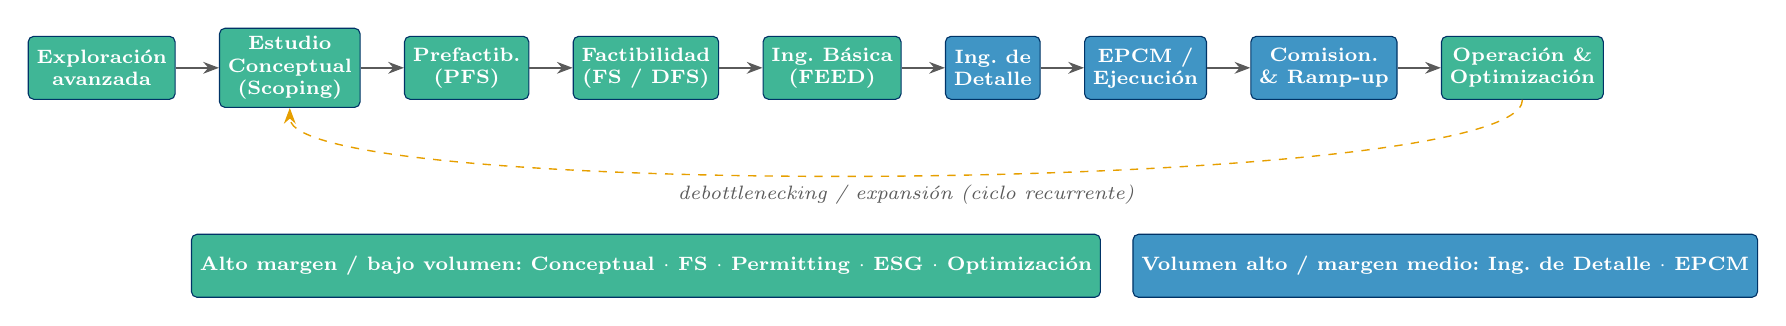
\begin{tikzpicture}[node distance=4.5mm and 5.5mm]
  \node[hibox] (ex) {Exploración\\avanzada};
  \node[hibox,right=of ex] (co) {Estudio\\Conceptual\\(Scoping)};
  \node[hibox,right=of co] (pf) {Prefactib.\\(PFS)};
  \node[hibox,right=of pf] (fs) {Factibilidad\\(FS / DFS)};
  \node[hibox,right=of fs] (be) {Ing. Básica\\(FEED)};
  \node[midbox,right=of be] (de) {Ing. de\\Detalle};
  \node[midbox,right=of de] (ep) {EPCM /\\Ejecución};
  \node[midbox,right=of ep] (cm) {Comision.\\\& Ramp-up};
  \node[hibox,right=of cm] (op) {Operación \&\\Optimización};
  \foreach \a/\b in {ex/co,co/pf,pf/fs,fs/be,be/de,de/ep,ep/cm,cm/op}{\draw[fl] (\a) -- (\b);}
  \draw[fl,dashed,accentorange] (op.south) .. controls +(0,-1.2) and +(0,-1.2) .. (co.south)
        node[midway,below,font=\scriptsize\itshape,text=darkgray]{debottlenecking / expansión (ciclo recurrente)};
  % Leyenda de margen
  \node[hibox,minimum width=6cm,below=1.7cm of fs.south,anchor=north] (l1)
      {Alto margen / bajo volumen:\ Conceptual $\cdot$ FS $\cdot$ Permitting $\cdot$ ESG $\cdot$ Optimización};
  \node[midbox,minimum width=6cm,right=4mm of l1] (l2)
      {Volumen alto / margen medio:\ Ing. de Detalle $\cdot$ EPCM};
\end{tikzpicture}}
\caption[Cadena de valor del servicio de ingeniería minera]{Cadena de valor del servicio de ingeniería minera. En verde, fases de
alto margen y diferenciación; en azul, fases de alto volumen y mayor exposición al ciclo de CAPEX. Elaboración propia.}
\label{fig:cadena}
\end{figure}

\section{Ecosistema y fronteras del mercado}
El ecosistema involucra cinco grupos de actores: (i) los \emph{owners} mineros (mayores y \emph{juniors}); (ii) las firmas de
ingeniería y consultoría (de las cuales REDCO forma parte); (iii) los OEM y contratistas de construcción; (iv) los financistas
(banca, \emph{streaming}, mercados de capital y agencias de crédito a la exportación); y (v) el entorno regulatorio-social
(Estados, comunidades, marcos ESG). El mercado de servicios se ubica \emph{aguas arriba} de la construcción física y captura su
valor de forma anticipada y persistente: una decisión de inversión (FID) favorable detona simultáneamente demanda de ingeniería
de detalle, EPCM y, posteriormente, optimización operacional durante toda la vida del activo.

%=============================================================================
\chapter{Eje A --- Alcance Geográfico}
\label{cap:geo}
%=============================================================================
Se evalúan siete mercados ---\textbf{Chile, Brasil, Argentina, Canadá, Europa del Este, Rusia y Estados Unidos}--- sobre seis
dimensiones de entorno/riesgo sistémico y seis dimensiones de madurez de la demanda de ingeniería. La comparación multivariable
se sintetiza en los radares de la Figura~\ref{fig:radar}; el detalle numérico completo (las siete geografías) se entrega en las
Tablas~\ref{tab:radar-riesgo} y~\ref{tab:radar-madurez}.

\section{Radares comparativos de mercado}
\begin{figure}[htbp]
\centering
\begin{minipage}{0.49\textwidth}\centering
\resizebox{\linewidth}{!}{%
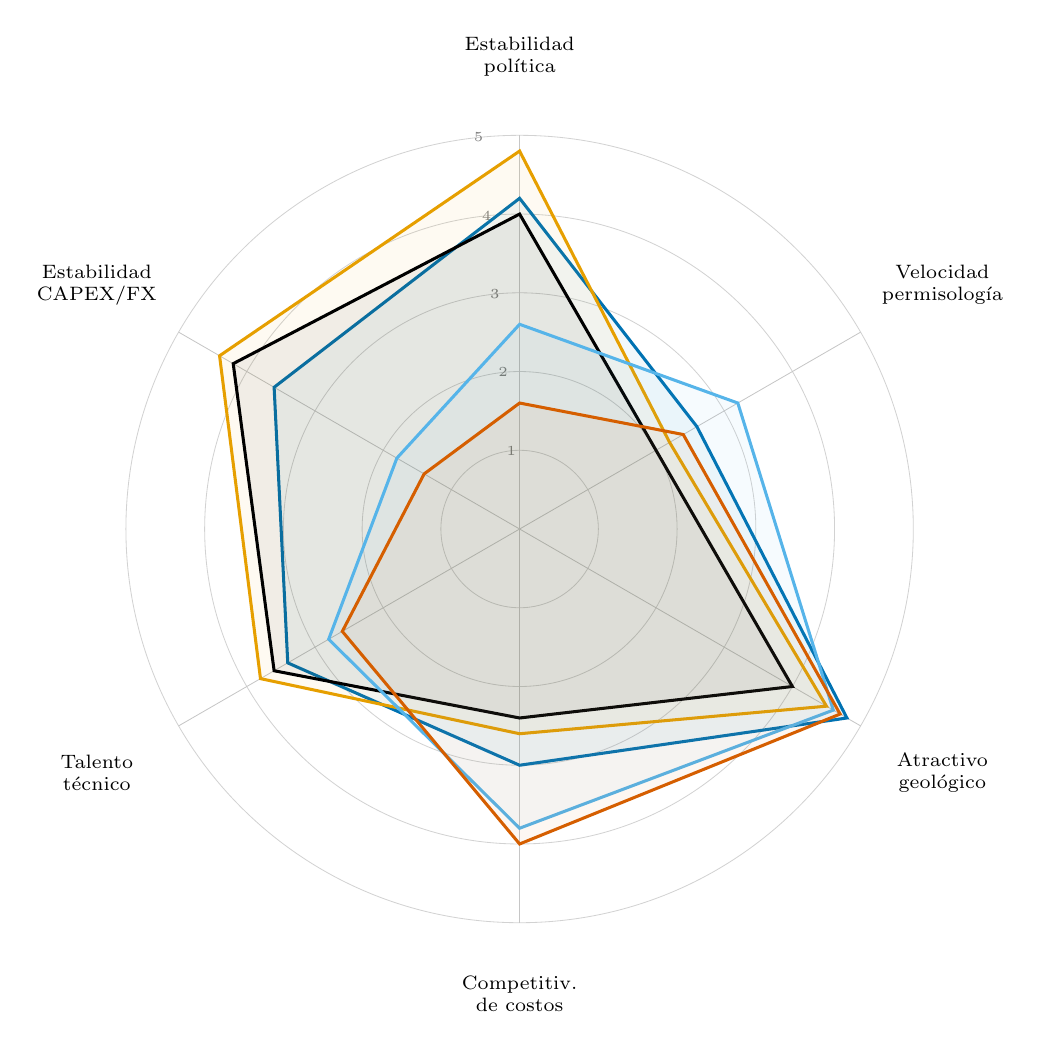
\begin{tikzpicture}[scale=1]
  \radargrid
  % Ejes: Estab.pol(90) Permisol(30) Atract.geol(-30) Costos(-90) Talento(-150) CAPEX/FX(150)
  \radarserie{accentblue}{4.2}{2.6}{4.8}{3.0}{3.4}{3.6}   % Chile
  \radarserie{accentorange}{4.8}{2.2}{4.5}{2.6}{3.8}{4.4} % Canadá
  \radarserie{black}{4.0}{2.0}{4.0}{2.4}{3.6}{4.2}        % EE.UU.
  \radarserie{accentsky}{2.6}{3.2}{4.6}{3.8}{2.8}{1.8}    % Argentina
  \radarserie{accentred}{1.6}{2.4}{4.7}{4.0}{2.6}{1.4}    % Rusia
  \node[font=\scriptsize,align=center] at (90:6.0) {Estabilidad\\política};
  \node[font=\scriptsize,align=center] at (30:6.2) {Velocidad\\permisología};
  \node[font=\scriptsize,align=center] at (-30:6.2) {Atractivo\\geológico};
  \node[font=\scriptsize,align=center] at (-90:5.9) {Competitiv.\\de costos};
  \node[font=\scriptsize,align=center] at (-150:6.2) {Talento\\técnico};
  \node[font=\scriptsize,align=center] at (150:6.2) {Estabilidad\\CAPEX/FX};
\end{tikzpicture}}
\\[2pt]{\scriptsize (a) Entorno / riesgo sistémico ($5=$ más favorable)}
\end{minipage}\hfill
\begin{minipage}{0.49\textwidth}\centering
\resizebox{\linewidth}{!}{%
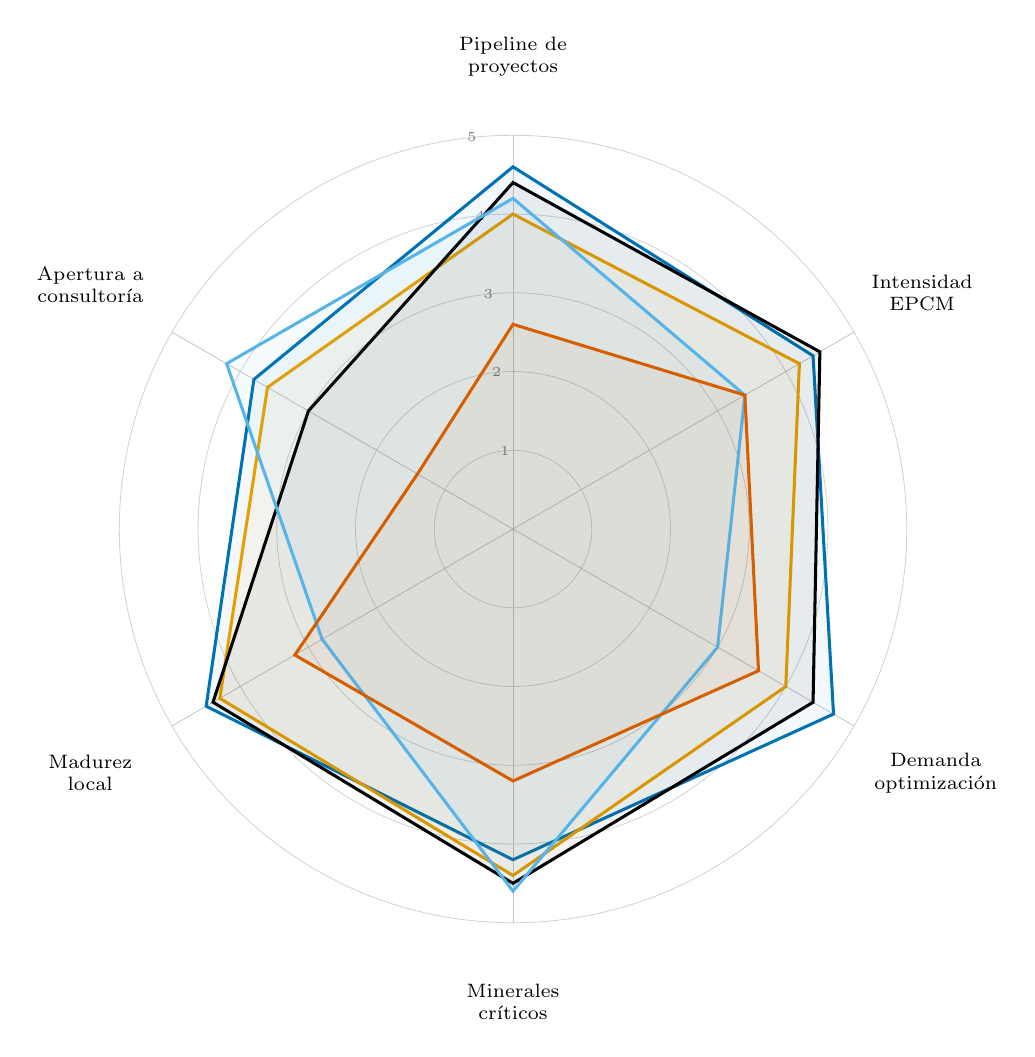
\begin{tikzpicture}[scale=1]
  \radargrid
  % Ejes: Pipeline(90) EPCM(30) Optim(-30) Min.crit(-90) Madurez loc(-150) Apertura(150)
  \radarserie{accentblue}{4.6}{4.4}{4.7}{4.2}{4.5}{3.8}   % Chile
  \radarserie{accentorange}{4.0}{4.2}{4.0}{4.4}{4.3}{3.6} % Canadá
  \radarserie{black}{4.4}{4.5}{4.4}{4.5}{4.4}{3.0}        % EE.UU.
  \radarserie{accentsky}{4.2}{3.4}{3.0}{4.6}{2.8}{4.2}    % Argentina
  \radarserie{accentred}{2.6}{3.4}{3.6}{3.2}{3.2}{1.4}    % Rusia
  \node[font=\scriptsize,align=center] at (90:6.0) {Pipeline de\\proyectos};
  \node[font=\scriptsize,align=center] at (30:6.0) {Intensidad\\EPCM};
  \node[font=\scriptsize,align=center] at (-30:6.2) {Demanda\\optimización};
  \node[font=\scriptsize,align=center] at (-90:6.0) {Minerales\\críticos};
  \node[font=\scriptsize,align=center] at (-150:6.2) {Madurez\\local};
  \node[font=\scriptsize,align=center] at (150:6.2) {Apertura a\\consultoría};
\end{tikzpicture}}
\\[2pt]{\scriptsize (b) Madurez de la demanda de ingeniería ($5=$ mayor tracción)}
\end{minipage}
\\[6pt]

\begin{tikzpicture}
\foreach \c/\n [count=\i] in {accentblue/Chile,accentorange/Canadá,black/EE.UU.,accentsky/Argentina,accentred/Rusia}{
  \node[anchor=west,font=\scriptsize] at ({(\i-1)*2.6},0) {\textcolor{\c}{\rule{6pt}{6pt}}~\n};}
\end{tikzpicture}
\caption[Radar comparativo de mercados de la gran minería]{Radares comparativos de cinco mercados representativos. En ambos
paneles, ``mayor $=$ más favorable para la firma de ingeniería''. Escala 1--5. Estimación del analista calibrada con indicadores
de gobernanza, \emph{pipeline} de proyectos y marcos de inversión. La matriz numérica de las siete geografías está en las
Tablas~\ref{tab:radar-riesgo} y~\ref{tab:radar-madurez}.}
\label{fig:radar}
\end{figure}

\section{Matriz comparativa de mercados}
\begin{table}[htbp]
\centering
\caption{Matriz comparativa de los siete mercados (cualitativa).}
\label{tab:mercados}
\scriptsize
\renewcommand{\arraystretch}{1.25}
\resizebox{\textwidth}{!}{%
\begin{tabular}{@{}lp{3.0cm}rcccl@{}}
\toprule
\rowcolor{tablehead}
\textcolor{white}{\textbf{Mercado}} & \textcolor{white}{\textbf{Minerales ancla}} &
\textcolor{white}{\textbf{CAPEX 24--30}} & \textcolor{white}{\textbf{Geología}} &
\textcolor{white}{\textbf{Gobernab.}} & \textcolor{white}{\textbf{Permisos}} &
\textcolor{white}{\textbf{Veredicto REDCO}}\\
\rowcolor{tablehead}
 & & \textcolor{white}{\footnotesize(USD mil M)} & & & \textcolor{white}{\footnotesize(años)} & \\
\midrule
\textbf{Chile} & Cobre, litio, molibdeno & 65--75 & Muy alto & Medio-alto & 8--12 & \textbf{Núcleo (Core)}\\
\rowcolor{tablealt}\textbf{Brasil} & Hierro, cobre, níquel, grafito, TR & 40--50 & Alto & Medio & 6--10 & Crecimiento\\
\textbf{Argentina} & Litio, cobre & 25--35 & Muy alto (Li) & Medio-bajo & 4--8 & Crecimiento (alta beta)\\
\rowcolor{tablealt}\textbf{Canadá} & Níquel, cobre, litio, uranio, TR & 45--55 & Muy alto & Muy alto & 10--15 & Expansión OCDE\\
\textbf{EE.UU.} & Cobre, litio, TR, grafito & 40--55 & Alto & Alto & 7--12 & Expansión OCDE\\
\rowcolor{tablealt}\textbf{Europa Este} & Cobre, níquel, litio, grafito & 15--25 & Medio & Medio & 6--10 & Selectivo / vía socios\\
\textbf{Rusia} & Níquel, paladio, cobre, oro, TR & n/d & Muy alto & Muy bajo & n/d & \textbf{Evitar / no-go}\\
\bottomrule
\end{tabular}}
\end{table}

\begin{cajahallazgo}[Lectura geográfica]
El ``corredor de las Américas'' (Chile + Argentina + Brasil + Canadá + EE.UU.) concentra la combinación más favorable de
geología, \emph{pipeline} de litio/cobre/níquel y acceso para firmas occidentales. \textbf{Rusia} mantiene dotaciones de
níquel-paladio de clase mundial, pero está \emph{fuera del conjunto factible} por sanciones y riesgo de contraparte/reputación:
cualquier exposición debe tratarse como \emph{no-go} para una firma con clientes y financistas OCDE. \textbf{Europa del Este} es un
mercado emergente de \emph{near-shoring} europeo (litio en Serbia/Chequia, cobre en Polonia) que conviene abordar vía
\emph{joint ventures} locales.
\end{cajahallazgo}

\section{\emph{Pipeline} de CAPEX por mercado}
\begin{figure}[htbp]
\centering
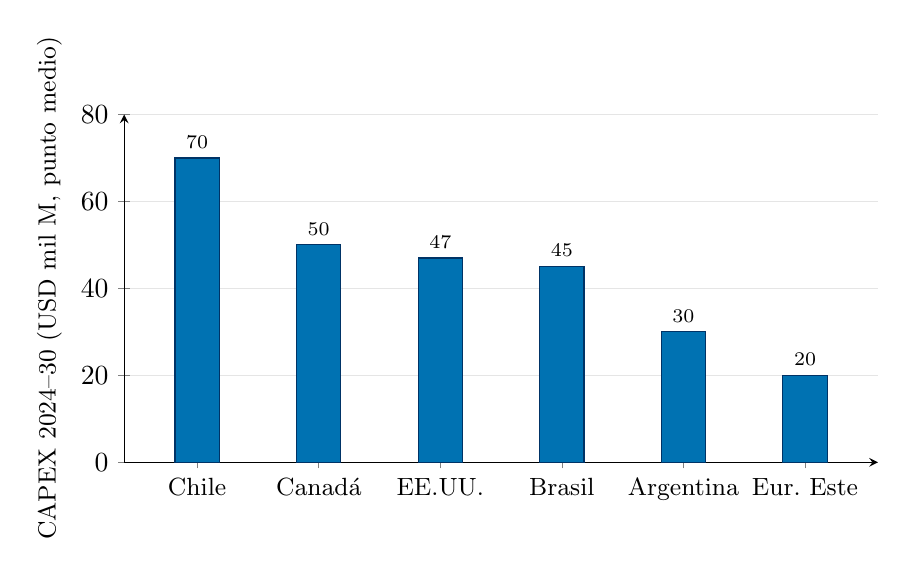
\begin{tikzpicture}
\begin{axis}[
  width=0.92\textwidth,height=6cm,
  ybar,bar width=16pt,
  ymin=0,ymax=80,
  ylabel={CAPEX 2024--30 (USD mil M, punto medio)},
  ylabel style={font=\small},
  xtick={1,2,3,4,5,6},
  xticklabels={Chile,Canadá,EE.UU.,Brasil,Argentina,Eur.\ Este},
  x tick label style={font=\small},
  xmin=0.4,xmax=6.6,
  nodes near coords,nodes near coords style={font=\scriptsize},
  every node near coord/.append style={anchor=south},
  bar shift=0,
  ymajorgrids,grid style={gray!20},
  axis lines=left]
\addplot[fill=accentblue,draw=primaryblue] coordinates
  {(1,70) (2,50) (3,47) (4,45) (5,30) (6,20)};
\end{axis}
\end{tikzpicture}
\caption[Pipeline de CAPEX minero por mercado]{\emph{Pipeline} estimado de CAPEX minero 2024--2030 por mercado (punto medio de
rango, orden de magnitud). Compárese con la Tabla~\ref{tab:mercados}. Elaboración propia con base en anuncios de proyectos
públicos y reportes de mineras \emph{majors}.}
\label{fig:capex-pais}
\end{figure}

\section{Concentración geográfica de la presión de demanda}
\begin{table}[htbp]
\centering
\caption{Geografías donde se concentra la presión de demanda de ingeniería al 2030, por mineral.}
\label{tab:geo-mineral}
\footnotesize
\renewcommand{\arraystretch}{1.2}
\begin{tabularx}{\textwidth}{@{}lX@{}}
\toprule
\rowcolor{tablehead}\textcolor{white}{\textbf{Mineral}} & \textcolor{white}{\textbf{Concentración geográfica de la presión de demanda}}\\
\midrule
Cobre & Chile, Perú (adyacente), EE.UU., Canadá, RD Congo/Zambia (fuera de alcance)\\
\rowcolor{tablealt}Litio & Argentina, Chile (salares), Canadá, EE.UU., Australia (fuera)\\
Níquel & Canadá, Brasil, Indonesia (fuera), Rusia (restringido)\\
\rowcolor{tablealt}Grafito & Brasil, Canadá, EE.UU. (ánodo doméstico), Mozambique (fuera)\\
Neodimio (TR) & EE.UU., Canadá, Brasil, Europa del Este\\
\rowcolor{tablealt}Plata & Chile, EE.UU., México (adyacente)\\
Acero / Aluminio (base) & Brasil (hierro), Canadá, EE.UU.\\
\bottomrule
\end{tabularx}
\end{table}

%=============================================================================
\chapter{Eje B --- Proyección de Demanda de Minerales al 2030}
\label{cap:minerales}
%=============================================================================
Se proyecta la demanda global para diez materiales. Las cifras son estimaciones trianguladas (rango $\rightarrow$ punto medio del
escenario base) calibradas con fuentes oficiales. El crecimiento se modela como:
\begin{equation}
D_{m,2030} \;=\; D_{m,2024}\,\bigl(1+g_m\bigr)^{6}, \qquad g_m=\text{CAGR de demanda del mineral } m.
\label{eq:demanda}
\end{equation}

\section{Tabla maestra de proyección (escenario base)}
\begin{table}[htbp]
\centering
\caption{Proyección de demanda 2024$\rightarrow$2030, escenario base. TR $=$ tierras raras; LCE $=$ \emph{lithium carbonate equivalent}.}
\label{tab:demanda-maestra}
\scriptsize
\renewcommand{\arraystretch}{1.25}
\resizebox{\textwidth}{!}{%
\begin{tabular}{@{}llrrrll@{}}
\toprule
\rowcolor{tablehead}
\textcolor{white}{\textbf{Mineral}} & \textcolor{white}{\textbf{Unidad}} &
\textcolor{white}{\textbf{2024}} & \textcolor{white}{\textbf{2030}} & \textcolor{white}{\textbf{CAGR}} &
\textcolor{white}{\textbf{Driver dominante}} & \textcolor{white}{\textbf{Intens. ing.}}\\
\midrule
\textbf{Litio}             & Mt LCE & 1{,}0  & 2{,}6  & $\sim$16\,\% & Baterías EV + BESS        & Muy alta\\
\rowcolor{tablealt}\textbf{Cobalto} & Mt & 0{,}20 & 0{,}27 & $\sim$5\,\%  & Baterías (NMC)            & Alta\\
\textbf{Grafito} (nat.+sint.) & Mt  & 5{,}5  & 8{,}5  & $\sim$7{,}5\,\% & Ánodos de batería       & Alta\\
\rowcolor{tablealt}\textbf{Níquel} & Mt & 3{,}3  & 4{,}3  & $\sim$4{,}5\,\% & Baterías + acero inox.  & Alta\\
\textbf{Neodimio} (NdPr imán) & kt  & 55     & 73     & $\sim$5\,\%  & Imanes (EV + eólica)      & Muy alta\\
\rowcolor{tablealt}\textbf{Silicio} (metal+poly) & Mt & 5{,}5 & 8{,}5 & $\sim$7{,}5\,\% & Solar PV + electrónica & Media-alta\\
\textbf{Cobre} (refinado)  & Mt     & 27{,}0 & 30{,}0 & $\sim$1{,}8\,\% & Redes + EV + edificación & Alta\\
\rowcolor{tablealt}\textbf{Plata} & kt & 36   & 44     & $\sim$3{,}4\,\% & Solar PV + electrónica  & Media\\
\textbf{Aluminio} (total)  & Mt     & 101    & 120    & $\sim$3\,\%  & Liviano EV + redes + constr. & Media\\
\rowcolor{tablealt}\textbf{Acero} (crudo) & Mt & 1\,880 & 1\,957 & $\sim$0{,}7\,\% & Construcción + infraestr. & Baja (por \$)\\
\bottomrule
\end{tabular}}
\end{table}

\begin{cajahallazgo}[Insight B --- el \emph{fee pool} crece más rápido que el tonelaje]
Los mayores multiplicadores de demanda (litio $\times 2{,}6$; grafito y TR $\sim\!\times 1{,}6$) coinciden con la mayor intensidad de
ingeniería. Cada tonelada incremental de litio o tierras raras requiere procesos novedosos (extracción directa de litio --- DLE,
separación de TR, hidrometalurgia) con alto contenido de estudios, pilotaje y FEED. En contraste, acero y aluminio dominan el
tonelaje, pero su demanda incremental es madura y de baja intensidad de ingeniería por dólar.
\end{cajahallazgo}

\section{Trayectoria indexada de demanda}
\begin{figure}[htbp]
\centering
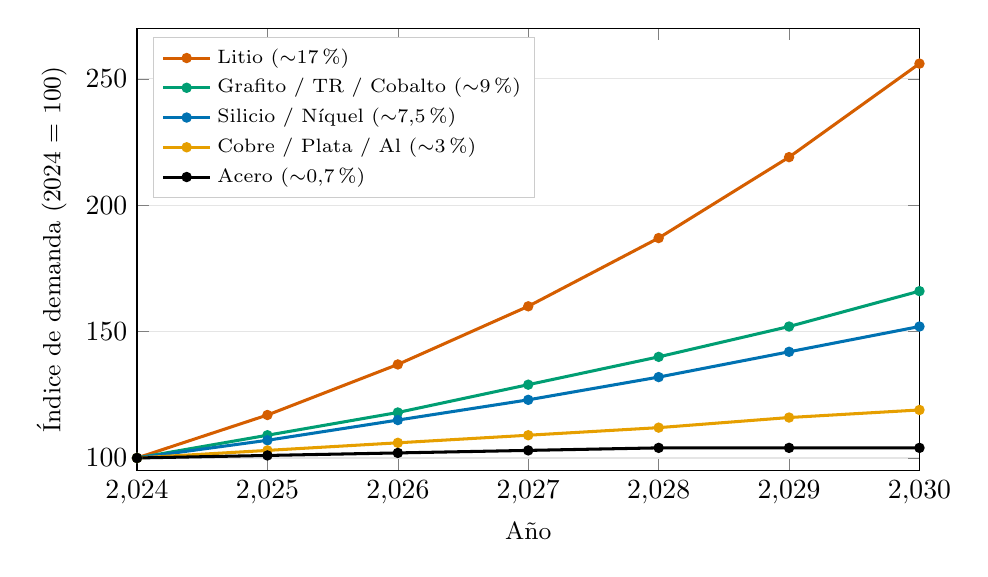
\begin{tikzpicture}
\begin{axis}[
  width=0.95\textwidth,height=7.2cm,
  xlabel={Año},ylabel={Índice de demanda (2024 $=$ 100)},
  xlabel style={font=\small},ylabel style={font=\small},
  xmin=2024,xmax=2030,ymin=95,ymax=270,
  xtick={2024,2025,2026,2027,2028,2029,2030},
  ymajorgrids,grid style={gray!20},
  legend style={font=\scriptsize,at={(0.02,0.98)},anchor=north west,draw=gray!40},
  legend cell align=left,
  every axis plot/.append style={line width=1.1pt,mark=*,mark size=1.3pt}]
\addplot[accentred]   coordinates {(2024,100)(2025,117)(2026,137)(2027,160)(2028,187)(2029,219)(2030,256)};
\addplot[accentgreen] coordinates {(2024,100)(2025,109)(2026,118)(2027,129)(2028,140)(2029,152)(2030,166)};
\addplot[accentblue]  coordinates {(2024,100)(2025,107)(2026,115)(2027,123)(2028,132)(2029,142)(2030,152)};
\addplot[accentorange]coordinates {(2024,100)(2025,103)(2026,106)(2027,109)(2028,112)(2029,116)(2030,119)};
\addplot[black]       coordinates {(2024,100)(2025,101)(2026,102)(2027,103)(2028,104)(2029,104)(2030,104)};
\legend{Litio ($\sim$17\,\%),Grafito / TR / Cobalto ($\sim$9\,\%),Silicio / Níquel ($\sim$7{,}5\,\%),Cobre / Plata / Al ($\sim$3\,\%),Acero ($\sim$0{,}7\,\%)}
\end{axis}
\end{tikzpicture}
\caption[Trayectoria indexada de demanda de minerales 2024--2030]{Trayectoria indexada de demanda (2024 $=$ 100), escenario base.
Las pendientes ilustran la divergencia entre minerales de batería (litio, grafito) y minerales base maduros (acero). Valores
absolutos en la Tabla~\ref{tab:demanda-maestra}. Fuentes: IEA~\cite{iea_gcmo2025}, OECD~\cite{oecd_steel2025}, IAI~\cite{iai_demand}.}
\label{fig:trayectoria}
\end{figure}

\section{Comparación de volúmenes por mineral}
\begin{figure}[htbp]
\centering
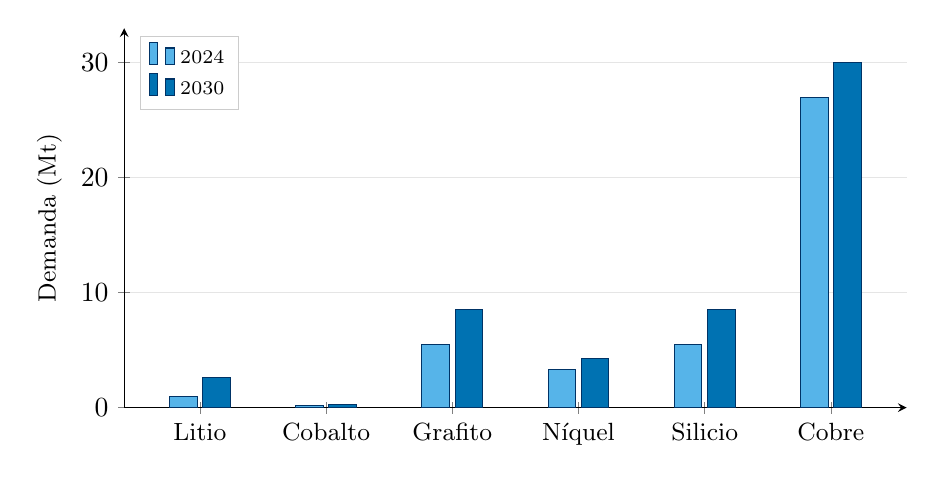
\begin{tikzpicture}
\begin{axis}[
  width=0.95\textwidth,height=6.4cm,
  ybar=2pt,bar width=10pt,
  ymin=0,ymax=33,
  ylabel={Demanda (Mt)},ylabel style={font=\small},
  xtick={1,2,3,4,5,6},xticklabels={Litio,Cobalto,Grafito,Níquel,Silicio,Cobre},
  x tick label style={font=\small},
  xmin=0.4,xmax=6.6,
  ymajorgrids,grid style={gray!20},axis lines=left,
  legend style={font=\scriptsize,at={(0.02,0.98)},anchor=north west,draw=gray!40}]
\addplot[fill=accentsky,draw=primaryblue] coordinates {(1,1.0)(2,0.20)(3,5.5)(4,3.3)(5,5.5)(6,27.0)};
\addplot[fill=accentblue,draw=primaryblue] coordinates {(1,2.6)(2,0.27)(3,8.5)(4,4.3)(5,8.5)(6,30.0)};
\legend{2024,2030}
\end{axis}
\end{tikzpicture}
\caption[Demanda 2024 vs.\ 2030 por mineral seleccionado]{Demanda 2024 (claro) vs.\ 2030 (oscuro), minerales en escala
comparable (Mt). Acero (1\,880$\rightarrow$1\,957 Mt), aluminio (101$\rightarrow$120 Mt) y plata/neodimio (en kt) se excluyen de
este eje por escala; véase la Tabla~\ref{tab:demanda-maestra}.}
\label{fig:barras-mineral}
\end{figure}

%=============================================================================
\chapter{Eje C --- Tracción de la Demanda}
\label{cap:traccion}
%=============================================================================
La relación causa-efecto entre las \textbf{tecnologías de transición} y las \textbf{necesidades de materiales} es el núcleo del
crecimiento secular. El mapa de la Figura~\ref{fig:traccion} establece qué tecnología tracciona cuál mineral y dónde se concentra
geográficamente la presión.

\section{Mapa de tracción: tecnologías $\rightarrow$ minerales $\rightarrow$ geografía}
\begin{figure}[htbp]
\centering
\resizebox{\textwidth}{!}{%
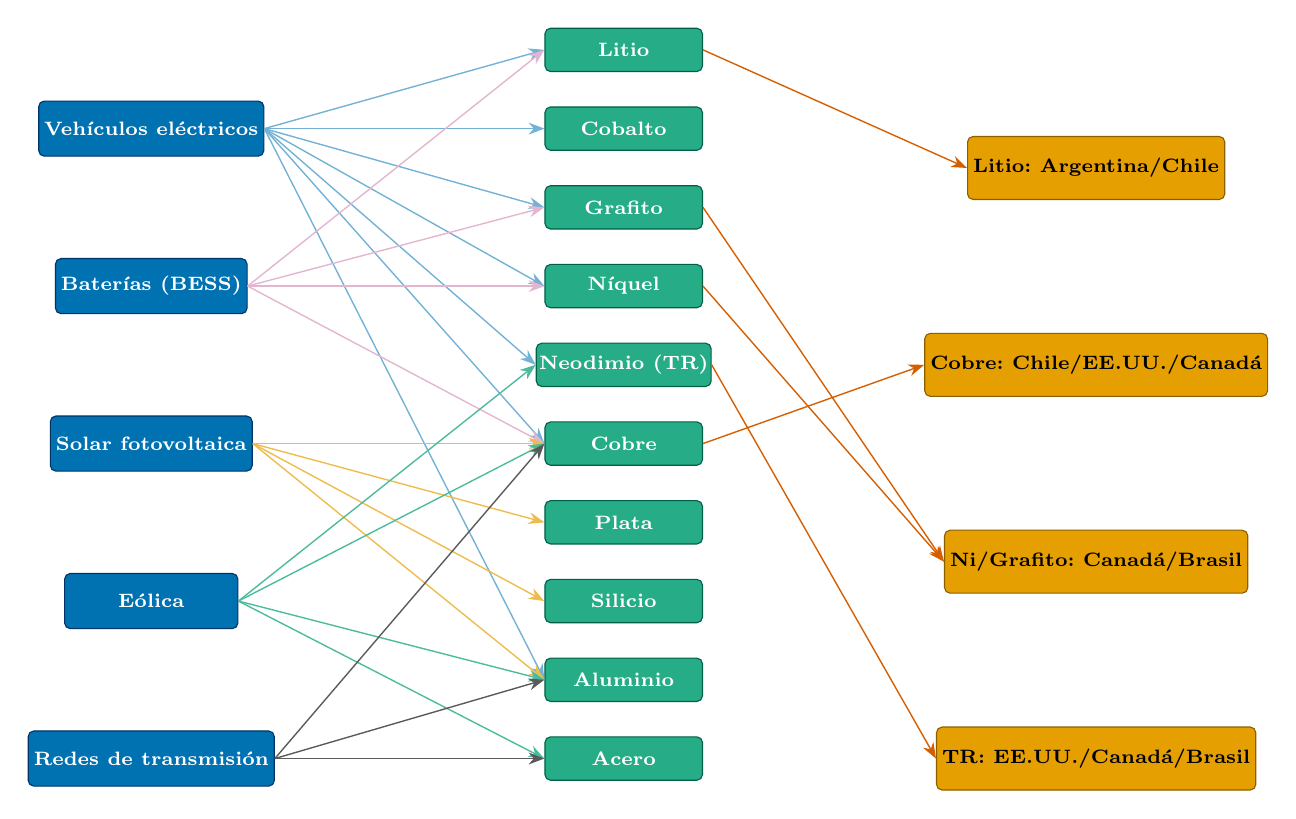
\begin{tikzpicture}[x=1cm,y=1cm]
  % --- Columna 1: tecnologías ---
  \node[techbox] (EV)   at (0,8) {Vehículos eléctricos};
  \node[techbox] (BAT)  at (0,6) {Baterías (BESS)};
  \node[techbox] (PV)   at (0,4) {Solar fotovoltaica};
  \node[techbox] (WIND) at (0,2) {Eólica};
  \node[techbox] (GRID) at (0,0) {Redes de transmisión};
  % --- Columna 2: materiales ---
  \foreach \name/\y/\lab in {LI/9/Litio,CO/8/Cobalto,GR/7/Grafito,NI/6/Níquel,ND/5/{Neodimio (TR)},CU/4/Cobre,AG/3/Plata,SI/2/Silicio,AL/1/Aluminio,FE/0/Acero}{
    \node[matbox] (\name) at (6,\y) {\lab};}
  % --- Columna 3: geografías ---
  \node[geobox] (G1) at (12,7.5) {Litio:\ Argentina/Chile};
  \node[geobox] (G2) at (12,5.0) {Cobre:\ Chile/EE.UU./Canadá};
  \node[geobox] (G3) at (12,2.5) {Ni/Grafito:\ Canadá/Brasil};
  \node[geobox] (G4) at (12,0.0) {TR:\ EE.UU./Canadá/Brasil};
  % --- Aristas tecnología -> material ---
  \foreach \d in {LI,CO,GR,NI,ND,CU,AL}{\draw[fl,accentblue!55] (EV.east) -- (\d.west);}
  \foreach \d in {LI,GR,NI,CU}{\draw[fl,accentpurple!55] (BAT.east) -- (\d.west);}
  \foreach \d in {SI,AG,CU,AL}{\draw[fl,accentorange!70] (PV.east) -- (\d.west);}
  \foreach \d in {ND,CU,FE,AL}{\draw[fl,accentgreen!70] (WIND.east) -- (\d.west);}
  \foreach \d in {CU,AL,FE}{\draw[fl,darkgray] (GRID.east) -- (\d.west);}
  % --- Aristas material -> geografía ---
  \draw[fl,accentred] (LI.east) -- (G1.west);
  \draw[fl,accentred] (CU.east) -- (G2.west);
  \draw[fl,accentred] (NI.east) -- (G3.west);
  \draw[fl,accentred] (GR.east) -- (G3.west);
  \draw[fl,accentred] (ND.east) -- (G4.west);
\end{tikzpicture}}
\caption[Mapa de tracción tecnologías $\rightarrow$ minerales $\rightarrow$ geografía]{Mapa de tracción de la demanda. Azul: EV;
magenta: BESS; naranja: solar PV; verde: eólica; gris: redes. En rojo, la canalización geográfica de la presión por mineral.
Solo se grafican las relaciones dominantes y relevantes ($\bullet\!\bullet$ o superior en la Tabla~\ref{tab:traccion}).}
\label{fig:traccion}
\end{figure}

\section{Matriz de tracción tecnología $\times$ mineral}
\begin{table}[htbp]
\centering
\caption{Intensidad de la tracción tecnología $\times$ mineral. $\bullet\bullet\bullet=$ driver dominante; $\bullet\bullet=$ relevante; $\bullet=$ secundario; --- $=$ no material.}
\label{tab:traccion}
\scriptsize
\renewcommand{\arraystretch}{1.3}
\resizebox{\textwidth}{!}{%
\begin{tabular}{@{}lcccccccccc@{}}
\toprule
\rowcolor{tablehead}
\textcolor{white}{\textbf{Tecnología} $\backslash$ \textbf{Mineral}} &
\textcolor{white}{Li} & \textcolor{white}{Co} & \textcolor{white}{Gr} & \textcolor{white}{Ni} &
\textcolor{white}{Nd} & \textcolor{white}{Cu} & \textcolor{white}{Ag} & \textcolor{white}{Si} &
\textcolor{white}{Al} & \textcolor{white}{Fe}\\
\midrule
Vehículos eléctricos & $\bullet\bullet\bullet$ & $\bullet\bullet\bullet$ & $\bullet\bullet\bullet$ & $\bullet\bullet\bullet$ & $\bullet\bullet\bullet$ & $\bullet\bullet$ & --- & --- & $\bullet\bullet$ & $\bullet$\\
\rowcolor{tablealt}Baterías (BESS) & $\bullet\bullet\bullet$ & $\bullet\bullet$ & $\bullet\bullet\bullet$ & $\bullet\bullet$ & --- & $\bullet\bullet$ & --- & --- & $\bullet$ & $\bullet$\\
Solar PV & --- & --- & --- & --- & --- & $\bullet\bullet$ & $\bullet\bullet\bullet$ & $\bullet\bullet\bullet$ & $\bullet\bullet$ & $\bullet$\\
\rowcolor{tablealt}Eólica & --- & --- & --- & --- & $\bullet\bullet\bullet$ & $\bullet\bullet\bullet$ & --- & --- & $\bullet\bullet$ & $\bullet\bullet\bullet$\\
Redes de transmisión & --- & --- & --- & --- & --- & $\bullet\bullet\bullet$ & --- & --- & $\bullet\bullet\bullet$ & $\bullet\bullet$\\
\bottomrule
\end{tabular}}
\end{table}

\begin{cajahallazgo}[Insight C --- el cobre como denominador común]
El \textbf{cobre} es el único material con tracción $\bullet\bullet$ o superior en \emph{las cinco} tecnologías: es el ``denominador
común'' de la electrificación y el activo más resiliente para una cartera de ingeniería. El litio, el cobalto y el grafito dependen
casi exclusivamente del \emph{cluster} EV + BESS (mayor \emph{upside}, pero mayor concentración de riesgo de demanda). El
\textbf{neodimio} está doblemente traccionado por EV (motores) y eólica (generadores), con oferta geográficamente concentrada
$\rightarrow$ cuello de botella estratégico.
\end{cajahallazgo}

\section{Cuantificación de la tracción}
\begin{table}[htbp]
\centering
\caption{Porcentaje de la demanda incremental 2024--2030 atribuible a la transición energética.}
\label{tab:traccion-pct}
\footnotesize
\renewcommand{\arraystretch}{1.15}
\begin{tabularx}{0.8\textwidth}{@{}Xr@{}}
\toprule
\rowcolor{tablehead}\textcolor{white}{\textbf{Mineral}} & \textcolor{white}{\textbf{\% atribuible a transición}}\\
\midrule
Litio & $\sim$85--90\,\%\\
\rowcolor{tablealt}Grafito & $\sim$70--80\,\%\\
Cobalto & $\sim$65--75\,\%\\
\rowcolor{tablealt}Neodimio & $\sim$60--70\,\%\\
Silicio & $\sim$50--60\,\% (PV)\\
\rowcolor{tablealt}Níquel & $\sim$45--55\,\%\\
Cobre & $\sim$40--50\,\%\\
\rowcolor{tablealt}Plata & $\sim$40--50\,\% (PV)\\
Aluminio & $\sim$25--35\,\%\\
\rowcolor{tablealt}Acero & $\sim$5--10\,\%\\
\bottomrule
\end{tabularx}
\end{table}

%=============================================================================
\chapter{Descomposición de los Servicios Demandados}
\label{cap:servicios}
%=============================================================================
El crecimiento de la demanda no es homogéneo entre \textbf{tipos de servicio}. La Figura~\ref{fig:treemap} descompone el
\emph{fee pool} 2030 (base $\approx$ USD~22 mil millones) como un \emph{tree map} cuyas áreas son proporcionales a la
participación de cada servicio; la Tabla~\ref{tab:servicios} compara su dinámica estructural.

\section{\emph{Tree map} de descomposición del \emph{fee pool}}
\begin{figure}[htbp]
\centering
\resizebox{0.96\textwidth}{!}{%
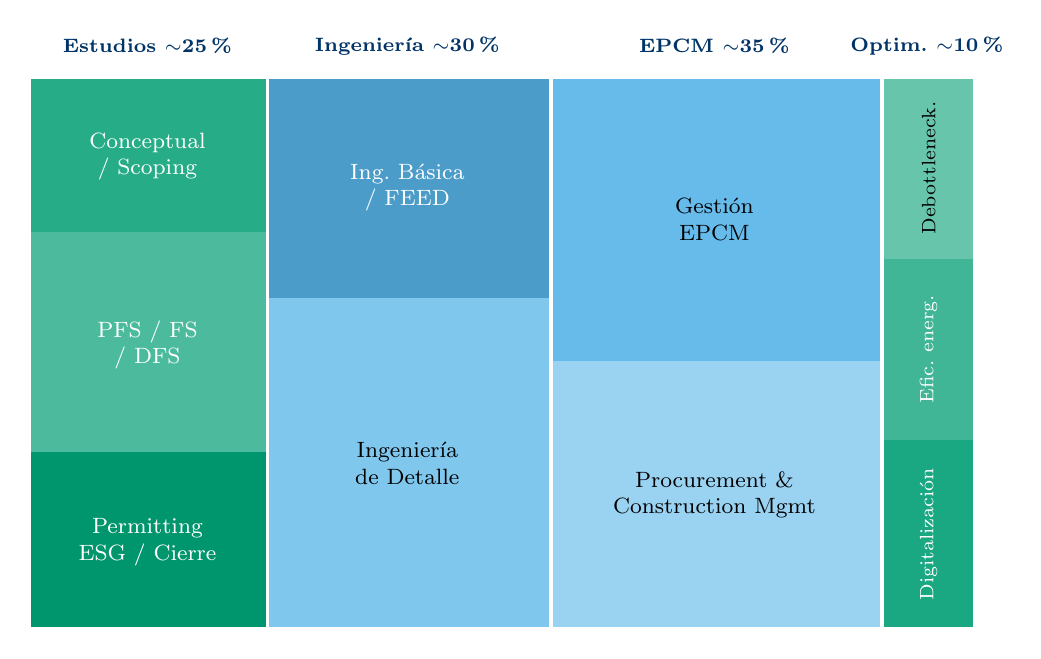
\begin{tikzpicture}[font=\footnotesize,every node/.style={align=center}]
  % Lienzo 12 x 7 ; colores por margen: verde=alto, azul=medio, celeste=bajo
  % --- Columna Estudios & Consultoría [0,3] (25%) ---
  \fill[accentgreen!85] (0,5.04) rectangle (3,7);        \node[white] at (1.5,6.0) {Conceptual\\/ Scoping};
  \fill[accentgreen!70] (0,2.24) rectangle (3,5.04);     \node[white] at (1.5,3.6) {PFS / FS\\/ DFS};
  \fill[accentgreen!95!black] (0,0) rectangle (3,2.24);  \node[white] at (1.5,1.1) {Permitting\\ESG / Cierre};
  % --- Columna Ingeniería [3.05,6.6] (30%) ---
  \fill[accentblue!70] (3.05,4.2) rectangle (6.6,7);     \node[white] at (4.8,5.6) {Ing. Básica\\/ FEED};
  \fill[accentsky!75] (3.05,0) rectangle (6.6,4.2);      \node[black] at (4.8,2.1) {Ingeniería\\de Detalle};
  % --- Columna EPCM / Ejecución [6.65,10.8] (35%) ---
  \fill[accentsky!90] (6.65,3.4) rectangle (10.8,7);     \node[black] at (8.7,5.2) {Gestión\\EPCM};
  \fill[accentsky!60] (6.65,0) rectangle (10.8,3.4);     \node[black] at (8.7,1.7) {Procurement \&\\Construction Mgmt};
  % --- Columna Optimización [10.85,12] (10%) ---
  \fill[accentgreen!60] (10.85,4.7) rectangle (12,7);    \node[black,rotate=90,font=\scriptsize] at (11.42,5.85) {Debottleneck.};
  \fill[accentgreen!75] (10.85,2.4) rectangle (12,4.7);  \node[white,rotate=90,font=\scriptsize] at (11.42,3.55) {Efic. energ.};
  \fill[accentgreen!90] (10.85,0) rectangle (12,2.4);    \node[white,rotate=90,font=\scriptsize] at (11.42,1.2) {Digitalización};
  % --- Encabezados de grupo ---
  \node[font=\scriptsize\bfseries,text=primaryblue] at (1.5,7.4)  {Estudios $\sim$25\,\%};
  \node[font=\scriptsize\bfseries,text=primaryblue] at (4.8,7.4)  {Ingeniería $\sim$30\,\%};
  \node[font=\scriptsize\bfseries,text=primaryblue] at (8.7,7.4)  {EPCM $\sim$35\,\%};
  \node[font=\scriptsize\bfseries,text=primaryblue] at (11.4,7.4) {Optim. $\sim$10\,\%};
  % marco
  \draw[white,line width=1.2pt] (0,0) rectangle (12,7);
\end{tikzpicture}}
\caption[Tree map de servicios de ingeniería minera]{\emph{Tree map} del \emph{fee pool} 2030 (base): el área es proporcional a
la participación de cada servicio. Verde $=$ alto margen; azul $=$ margen medio; celeste $=$ margen medio-bajo / alta competencia
de precio. Elaboración propia.}
\label{fig:treemap}
\end{figure}

\section{EPCM vs.\ Conceptual vs.\ Detalle: comparación estructural}
\begin{table}[htbp]
\centering
\caption{Comparación estructural por tipo de servicio.}
\label{tab:servicios}
\footnotesize
\renewcommand{\arraystretch}{1.3}
\resizebox{\textwidth}{!}{%
\begin{tabular}{@{}lcccc@{}}
\toprule
\rowcolor{tablehead}
\textcolor{white}{\textbf{Dimensión}} & \textcolor{white}{\textbf{Estudios / Concept.}} &
\textcolor{white}{\textbf{Ing. de Detalle}} & \textcolor{white}{\textbf{EPCM / Ejecución}} &
\textcolor{white}{\textbf{Optimización}}\\
\midrule
\% del \emph{fee pool} 2030 & $\sim$25\,\% & $\sim$18\,\% & $\sim$35\,\% & $\sim$10\,\%\\
\rowcolor{tablealt}Margen relativo & \textbf{Alto} & Medio-bajo & Medio & \textbf{Alto}\\
Ciclicidad & Anticíclico/temprano & Procíclico & \textbf{Muy procíclico} & Anticíclico\\
\rowcolor{tablealt}Barrera de entrada & Alta & Baja-media & Alta & Media-alta\\
Exposición a CAPEX & Baja & Media & \textbf{Muy alta} & Baja\\
\rowcolor{tablealt}Diferenciación REDCO & \textbf{Alta} & Baja & Media & \textbf{Alta}\\
\bottomrule
\end{tabular}}
\end{table}

\begin{cajahallazgo}[Insight de cartera de servicios]
Una cartera resiliente combina \textbf{estudios + optimización} (anticíclicos, alto margen, defienden ingresos en la baja del
ciclo) con una exposición \emph{medida} a EPCM (procíclico, capturador de volumen en la alta). El segmento de
\emph{permitting}/ESG es el de mayor crecimiento de margen porque la permisología se ha vuelto la restricción dominante
(véase Capítulo~\ref{cap:riesgos}).
\end{cajahallazgo}

%=============================================================================
\chapter{Eje D --- Riesgos Sistémicos y Mitigación}
\label{cap:riesgos}
%=============================================================================
Se evalúan los riesgos para el \textbf{negocio de la consultoría de ingeniería minera} (no para el minero \emph{owner}), puntuando
\textbf{probabilidad} ($P$) e \textbf{impacto} ($I$) en escala 1--5. La \textbf{severidad} es $S = P \times I$ (máximo 25).

\section{Registro de riesgos}
\begin{table}[htbp]
\centering
\caption{Registro de riesgos del negocio de ingeniería minera (\emph{risk register}).}
\label{tab:riesgos}
\scriptsize
\renewcommand{\arraystretch}{1.25}
\resizebox{\textwidth}{!}{%
\begin{tabular}{@{}clccccp{5.4cm}@{}}
\toprule
\rowcolor{tablehead}
\textcolor{white}{\textbf{ID}} & \textcolor{white}{\textbf{Riesgo}} & \textcolor{white}{\textbf{Categoría}} &
\textcolor{white}{$P$} & \textcolor{white}{$I$} & \textcolor{white}{$S$} & \textcolor{white}{\textbf{Mitigación}}\\
\midrule
R1 & Sanciones / bloqueo geopolítico & Geopolítico & 4 & 5 & \textbf{20} & Ring-fencing; no-go en Rusia; \emph{due diligence} de contraparte; fuerza mayor\\
\rowcolor{tablealt}R2 & Retrasos de permisología & Regulatorio & 5 & 4 & \textbf{20} & Capacidad de \emph{permitting}/ESG; contratos por fases; \emph{milestone billing}\\
R3 & Escasez de talento técnico senior & Operacional & 5 & 4 & \textbf{20} & Plan de talento; ingeniería digital; centros de entrega; alianzas universitarias\\
\rowcolor{tablealt}R4 & Volatilidad de CAPEX & Financiero & 4 & 4 & \textbf{16} & Mix \emph{reimbursable+incentive}; cartera estudios$\leftrightarrow$EPCM; \emph{backlog} diversificado\\
R6 & Oposición comunitaria / licencia social & Social/ESG & 4 & 4 & \textbf{16} & \emph{Stakeholder engineering}; diseño \emph{water-positive}; ESG temprano\\
\rowcolor{tablealt}R5 & Inflación de costos y FX & Macroeconóm. & 4 & 3 & \textbf{12} & \emph{Pricing} en USD; cláusulas de escalamiento; cobertura FX\\
R8 & Concentración de cliente / contraparte & Comercial & 3 & 4 & \textbf{12} & Diversificación por cliente, país y mineral\\
\rowcolor{tablealt}R10 & Riesgo cambiario y de repatriación & Financiero & 3 & 4 & \textbf{12} & Cobro \emph{offshore}; límites de exposición por país\\
R7 & Disrupción tecnológica de proceso & Tecnológico & 3 & 3 & \textbf{9} & I+D; \emph{partnerships}; capacidad de pilotaje\\
\rowcolor{tablealt}R9 & Cambio fiscal / \emph{royalties} & Regulatorio & 3 & 3 & \textbf{9} & Monitoreo regulatorio; flexibilidad de modelos financieros\\
R11 & Ciberseguridad / pérdida de IP & Operacional & 3 & 3 & \textbf{9} & Gobernanza de datos; segregación de entornos; ciberseguros\\
\rowcolor{tablealt}R12 & Descarbonización forzada & Regul./ESG & 3 & 3 & \textbf{9} & Capacidad en eficiencia energética y electrificación de faena\\
\bottomrule
\end{tabular}}
\end{table}

\section{Distribución de frecuencia de riesgos}
\begin{figure}[htbp]
\centering
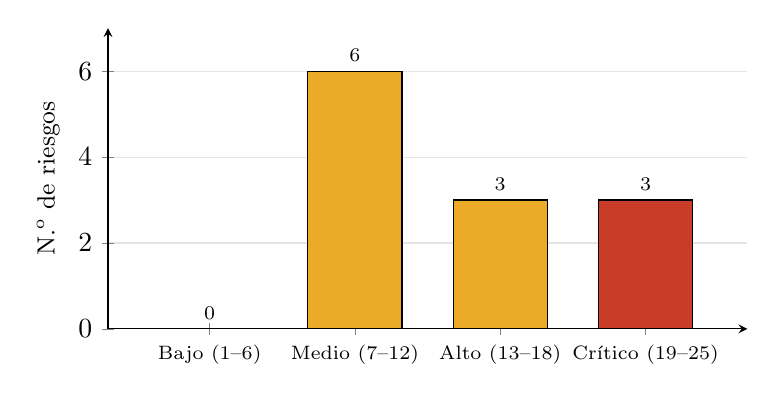
\begin{tikzpicture}
\begin{axis}[
  width=0.8\textwidth,height=5.4cm,
  ybar,bar width=34pt,
  ymin=0,ymax=7,
  ylabel={N.\textsuperscript{o} de riesgos},ylabel style={font=\small},
  xtick={1,2,3,4},
  xticklabels={{Bajo (1--6)},{Medio (7--12)},{Alto (13--18)},{Crítico (19--25)}},
  x tick label style={font=\scriptsize},
  xmin=0.3,xmax=4.7,
  nodes near coords,nodes near coords style={font=\scriptsize},
  bar shift=0,
  ymajorgrids,grid style={gray!20},axis lines=left]
\addplot[fill=risklo,draw=black] coordinates {(1,0)};
\addplot[fill=riskmed,draw=black,forget plot] coordinates {(2,6)};
\addplot[fill=riskmed,draw=black,forget plot] coordinates {(3,3)};
\addplot[fill=riskhi,draw=black,forget plot] coordinates {(4,3)};
\end{axis}
\end{tikzpicture}
\caption[Distribución de frecuencia de riesgos por severidad]{Distribución de frecuencia de los 12 riesgos por banda de
severidad $S=P\times I$. La masa se concentra en las bandas media y alta-crítica. Elaboración propia.}
\label{fig:hist-riesgo}
\end{figure}

\section{Mapa de calor de riesgos (Probabilidad \texorpdfstring{$\times$}{x} Impacto)}
\begin{figure}[htbp]
\centering
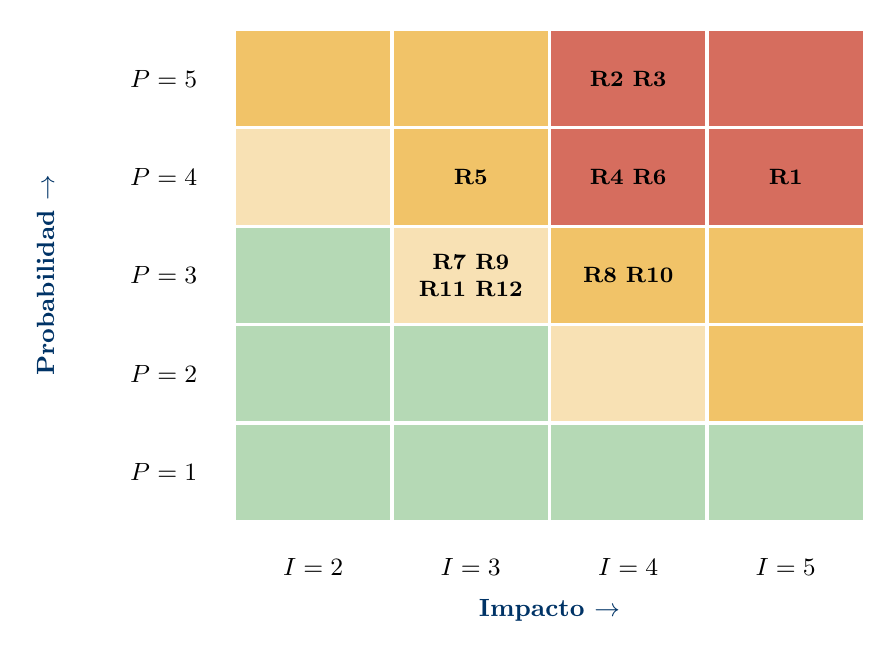
\begin{tikzpicture}[x=2.0cm,y=1.25cm,font=\footnotesize]
  % Celdas coloreadas por severidad S=P*I, P en filas (1..5 abajo->arriba), I en cols (2..5)
  \foreach \I in {2,3,4,5}{
    \foreach \P in {1,2,3,4,5}{
      \pgfmathtruncatemacro{\sev}{\I*\P}
      \ifnum\sev>15 \def\cc{riskhi!75}\else
        \ifnum\sev>9 \def\cc{riskmed!70}\else
          \ifnum\sev>6 \def\cc{riskmed!35}\else \def\cc{risklo!45}\fi\fi\fi
      \fill[\cc,draw=white,line width=1.2pt] (\I-0.5,\P-0.5) rectangle (\I+0.5,\P+0.5);
    }}
  % Etiquetas de riesgos en sus celdas (I,P)
  \node at (5,4) {\textbf{R1}};
  \node at (4,5) {\textbf{R2 R3}};
  \node at (4,4) {\textbf{R4 R6}};
  \node at (3,4) {\textbf{R5}};
  \node at (4,3) {\textbf{R8 R10}};
  \node[align=center] at (3,3) {\textbf{R7 R9}\\\textbf{R11 R12}};
  % Ejes
  \foreach \I in {2,3,4,5}{\node[below=10pt,font=\small] at (\I,0.5) {$I=\I$};}
  \foreach \P in {1,2,3,4,5}{\node[left=10pt,font=\small] at (1.5,\P) {$P=\P$};}
  \node[font=\small\bfseries,text=primaryblue] at (3.5,-0.4) {Impacto $\rightarrow$};
  \node[font=\small\bfseries,text=primaryblue,rotate=90] at (0.3,3) {Probabilidad $\rightarrow$};
\end{tikzpicture}
\caption[Mapa de calor de riesgos probabilidad $\times$ impacto]{Mapa de calor de riesgos. Verde $=$ severidad baja; ámbar $=$
media; rojo $=$ alta/crítica ($S\ge 16$). La zona crítica la ocupan R1 (geopolítica), R2 (permisología) y R3 (talento), que definen
la agenda de mitigación prioritaria. Cada celda corresponde a un par $(I,P)$.}
\label{fig:heatmap}
\end{figure}

\begin{cajariesgo}[Insight D --- el riesgo es de ejecución, no de demanda]
Los tres riesgos de mayor severidad (\textbf{R1 geopolítica, R2 permisología, R3 talento}) no son de demanda, sino de
\emph{ejecución y entorno}. La demanda secular está prácticamente asegurada por la transición energética; el riesgo real es la
capacidad de \textbf{convertir \emph{pipeline} en ingeniería facturada}. La firma que resuelva permisos + talento captura la renta
de escasez.
\end{cajariesgo}

%=============================================================================
\chapter{Eje E --- Proyecciones Financieras y Sensibilidad}
\label{cap:financiero}
%=============================================================================

\section{Modelo de valoración del mercado de servicios}
\label{sec:caveat}
\begin{cajanota}[Caveat sobre la cifra de mercado de servicios]
No existe una serie pública limpia y consensuada para el \emph{fee pool} exclusivo de ingeniería + consultoría minera. Las fuentes
disponibles miden objetos distintos: el mercado \textbf{EPCM global (todos los sectores)} se estima en $\sim$USD~5{,}4 mil millones
(2025), creciendo a $\sim$8{,}4\,\% CAGR, con el segmento minero en $\sim$USD~1{,}2 mil millones~\cite{epcm_market}. Por ello, la
cifra de \textbf{USD~$\sim$14 mil millones (2024) $\rightarrow$ $\sim$22 mil millones (2030)} es una \textbf{estimación propia
construida} como (CAPEX minero global $\sim$USD~120--150 mil millones/año) $\times$ (fracción de ingeniería + consultoría
$\sim$6--8\,\%) más consultoría de optimización sobre OPEX. La CAGR base $\sim$8\,\% es consistente con la del mercado EPCM
verificado. Trátese como orden de magnitud para decisión estratégica, no como dato citable a terceros.
\end{cajanota}

El valor del mercado de servicios al 2030 se modela como función del CAPEX minero, la fracción de ingeniería y un factor de
fricción de ejecución (permisos/talento):
\begin{equation}
V_{svc,2030} \;=\; \Bigl(\textstyle\sum_{m} \mathrm{CAPEX}_{m}\cdot \theta_{eng,m}\Bigr)\cdot \phi_{exec}
              \;+\; \theta_{op}\cdot \mathrm{OPEX}_{int}
\label{eq:vsvc}
\end{equation}
donde $\mathrm{CAPEX}_m$ es la inversión en proyectos del mineral $m$; $\theta_{eng,m}\in[0{,}04,0{,}07]$ la fracción de
ingeniería sobre CAPEX; $\phi_{exec}\in(0,1]$ el factor de ejecución (cuánto del \emph{pipeline} se convierte en gasto de
ingeniería, dados permisos y talento); y $\theta_{op}\cdot\mathrm{OPEX}_{int}$ la consultoría de optimización. El CAPEX por mineral
se aproxima con la nueva capacidad requerida y la intensidad de capital $\kappa_m$:
\begin{equation}
\mathrm{CAPEX}_{m} \;=\; \Delta C_{m}\cdot \kappa_{m},
\qquad \Delta C_{m} = \bigl(D_{m,2030}-D_{m,2024}\bigr)\cdot \frac{1}{u_m},
\label{eq:capexm}
\end{equation}
con $u_m$ el factor de utilización. La caída secular de leyes eleva $\kappa_m$ en el tiempo:
\begin{equation}
\kappa_{m}(t) \;=\; \kappa_{m,0}\cdot\Bigl(\tfrac{\bar g_0}{\bar g_t}\Bigr)^{\beta}, \qquad \beta>0,
\label{eq:kappa}
\end{equation}
donde $\bar g_t$ es la ley media del mineral en el año $t$: a menor ley, mayor CAPEX e ingeniería por tonelada.

\section{Definición de escenarios}
La trayectoria del valor se proyecta como producto de tasas anuales por escenario:
\begin{equation}
V_{svc,2030}^{(s)} \;=\; V_{2024}\cdot\prod_{t=2025}^{2030}\bigl(1+g_t^{(s)}\bigr),
\qquad s\in\{\text{Base},\text{Optimista},\text{Pesimista}\}.
\label{eq:escenarios}
\end{equation}

\begin{table}[htbp]
\centering
\caption{Parámetros y resultado por escenario.}
\label{tab:escenarios}
\footnotesize
\renewcommand{\arraystretch}{1.3}
\begin{tabularx}{\textwidth}{@{}Xccc@{}}
\toprule
\rowcolor{tablehead}
\textcolor{white}{\textbf{Parámetro}} & \textcolor{white}{\textbf{Pesimista}} &
\textcolor{white}{\textbf{Base}} & \textcolor{white}{\textbf{Optimista}}\\
\rowcolor{tablehead}
 & \textcolor{white}{\footnotesize Fragmentación} & \textcolor{white}{\footnotesize Transición gradual} & \textcolor{white}{\footnotesize Aceleración Net-Zero}\\
\midrule
CAGR de servicios $g^{(s)}$ & $\sim$3{,}5\,\% & \textbf{$\sim$8\,\%} & $\sim$13\,\%\\
\rowcolor{tablealt}Factor de ejecución $\phi_{exec}$ & 0{,}70 & 0{,}85 & 0{,}95\\
$\theta_{eng}$ medio & 0{,}045 & 0{,}055 & 0{,}065\\
\rowcolor{tablealt}Prima de riesgo geopolítico & Alta & Media & Baja\\
\textbf{Valor de mercado 2030 (USD)} & \textbf{$\sim$17 mil M} & \textbf{$\sim$22 mil M} & \textbf{$\sim$29 mil M}\\
\bottomrule
\end{tabularx}
\end{table}

\begin{description}[leftmargin=1.2em,style=nextline]
\item[Base --- Transición Gradual.] La electrificación avanza al ritmo planificado; la permisología sigue siendo el cuello de
  botella, pero gestionable; el CAPEX crece de forma sostenida. \emph{Fee pool} $\approx$ USD~22 mil millones.
\item[Optimista --- Aceleración Net-Zero.] Políticas de incentivo (IRA de EE.UU., CRMA de la UE, \emph{friend-shoring}) y precios
  firmes detonan una ola de FID; $\phi_{exec}$ y $\theta_{eng}$ suben. \emph{Fee pool} $\approx$ USD~29 mil millones.
\item[Pesimista --- Fragmentación y Proteccionismo.] Guerras comerciales, sobreoferta china de procesados, caída de precios de
  litio/níquel y diferimiento masivo de FID; la prima de riesgo eleva el costo de capital del \emph{owner}.
  \emph{Fee pool} $\approx$ USD~17 mil millones.
\end{description}

\section{Proyección del valor de mercado por escenario}
\begin{figure}[htbp]
\centering
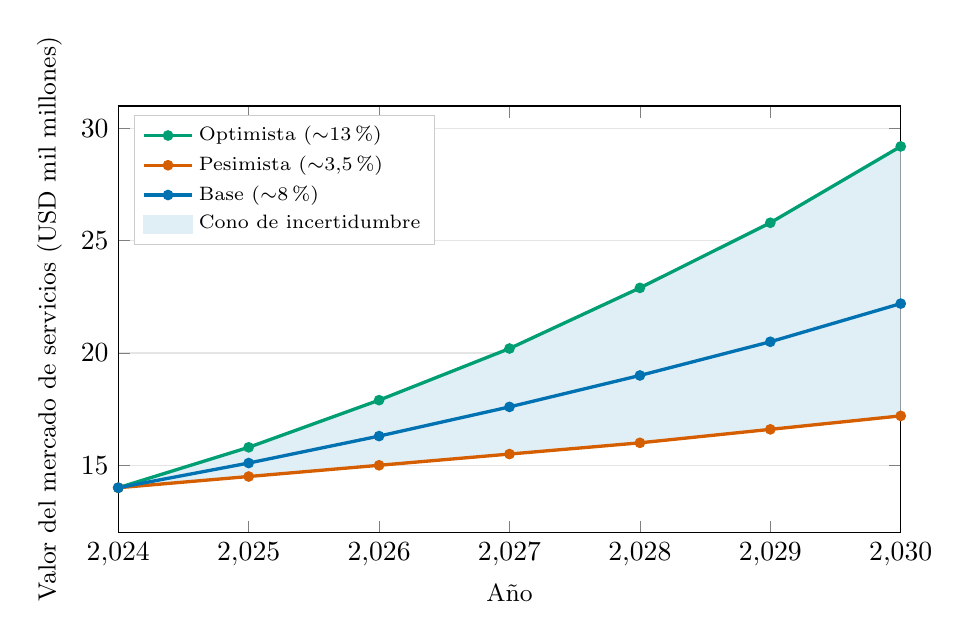
\begin{tikzpicture}
\begin{axis}[
  width=0.95\textwidth,height=7cm,
  xlabel={Año},ylabel={Valor del mercado de servicios (USD mil millones)},
  xlabel style={font=\small},ylabel style={font=\small},
  xmin=2024,xmax=2030,ymin=12,ymax=31,
  xtick={2024,2025,2026,2027,2028,2029,2030},
  ymajorgrids,grid style={gray!20},
  legend style={font=\scriptsize,at={(0.02,0.98)},anchor=north west,draw=gray!40},
  legend cell align=left,
  every axis plot/.append style={line width=1.2pt,mark=*,mark size=1.3pt}]
\addplot[name path=opt,accentgreen] coordinates {(2024,14)(2025,15.8)(2026,17.9)(2027,20.2)(2028,22.9)(2029,25.8)(2030,29.2)};
\addplot[name path=pes,accentred]   coordinates {(2024,14)(2025,14.5)(2026,15.0)(2027,15.5)(2028,16.0)(2029,16.6)(2030,17.2)};
\addplot[accentblue]                coordinates {(2024,14)(2025,15.1)(2026,16.3)(2027,17.6)(2028,19.0)(2029,20.5)(2030,22.2)};
\addplot[accentblue!12] fill between[of=opt and pes];
\legend{Optimista ($\sim$13\,\%),Pesimista ($\sim$3{,}5\,\%),Base ($\sim$8\,\%),Cono de incertidumbre}
\end{axis}
\end{tikzpicture}
\caption[Proyección del valor de mercado de servicios por escenario]{Valor del mercado de servicios de ingeniería minera, tres
escenarios (USD mil millones). El ``cono de incertidumbre'' entre la curva optimista y la pesimista asciende a $\sim$USD~12 mil
millones al 2030. Estimación construida (véase \S\ref{sec:caveat}).}
\label{fig:escenarios}
\end{figure}

\section{Análisis de sensibilidad (tornado)}
La Figura~\ref{fig:tornado} muestra el impacto sobre el valor base 2030 (USD~22 mil M) al variar cada \emph{driver}
$\pm 1$ desviación razonable, \emph{ceteris paribus}.
\begin{figure}[htbp]
\centering
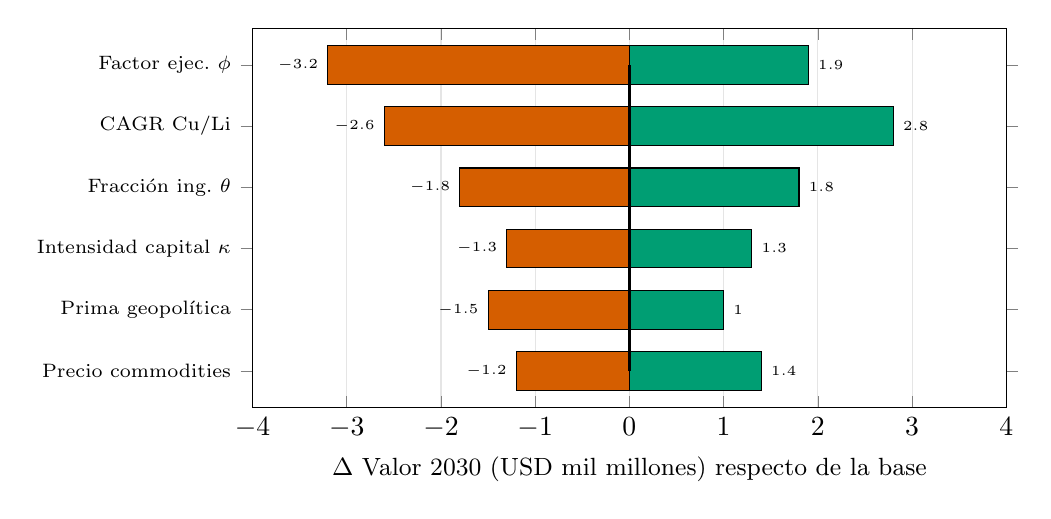
\begin{tikzpicture}
\begin{axis}[
  width=0.92\textwidth,height=6.4cm,
  xbar,bar width=14pt,
  xmin=-4,xmax=4,
  xlabel={$\Delta$ Valor 2030 (USD mil millones) respecto de la base},xlabel style={font=\small},
  ytick={1,2,3,4,5,6},
  yticklabels={Precio commodities,Prima geopolítica,Intensidad capital $\kappa$,Fracción ing.\ $\theta$,CAGR Cu/Li,Factor ejec.\ $\phi$},
  y tick label style={font=\scriptsize},
  ymin=0.4,ymax=6.6,
  nodes near coords,nodes near coords style={font=\tiny},
  every axis plot/.append style={bar shift=0},
  xmajorgrids,grid style={gray!20}]
\addplot[fill=accentred,draw=black] coordinates
  {(-3.2,6) (-2.6,5) (-1.8,4) (-1.3,3) (-1.5,2) (-1.2,1)};
\addplot[fill=accentgreen,draw=black] coordinates
  {(1.9,6) (2.8,5) (1.8,4) (1.3,3) (1.0,2) (1.4,1)};
\draw[black,thick] (axis cs:0,1) -- (axis cs:0,6);
\end{axis}
\end{tikzpicture}
\caption[Análisis de sensibilidad tornado]{Tornado de sensibilidad sobre el valor base 2030. Rojo $=$ desviación a la baja;
verde $=$ al alza. El \emph{driver} de mayor sensibilidad es el factor de ejecución $\phi_{exec}$ (permisos/talento), no el precio
del \emph{commodity}. Elaboración propia.}
\label{fig:tornado}
\end{figure}

\begin{cajahallazgo}[Insight E --- gestionar por $\phi_{exec}$, no por precio]
La palanca de mayor sensibilidad \emph{no} es el precio del \emph{commodity}, sino $\phi_{exec}$: la capacidad de convertir
\emph{pipeline} en ingeniería facturada (permisos + talento). Esto confirma la tesis del informe: el valor lo captura quien
resuelve el cuello de botella de ejecución, no quien apuesta al ciclo de precios.
\end{cajahallazgo}

\section{Correlación: ley del mineral vs.\ CAPEX de ingeniería}
La Figura~\ref{fig:scatter} relaciona la \textbf{ley media del yacimiento} (eje $X$, índice 0--100, mayor $=$ mejor ley) con el
\textbf{CAPEX de ingeniería por tonelada de capacidad} (eje $Y$, índice, mayor $=$ más intensivo). El ajuste lineal por mínimos
cuadrados sobre los nueve arquetipos de proyecto es:
\begin{equation}
Y \;\approx\; 102{,}5 \;-\; 0{,}97\,X, \qquad R^{2}\approx 0{,}79.
\label{eq:regresion}
\end{equation}
\begin{figure}[htbp]
\centering
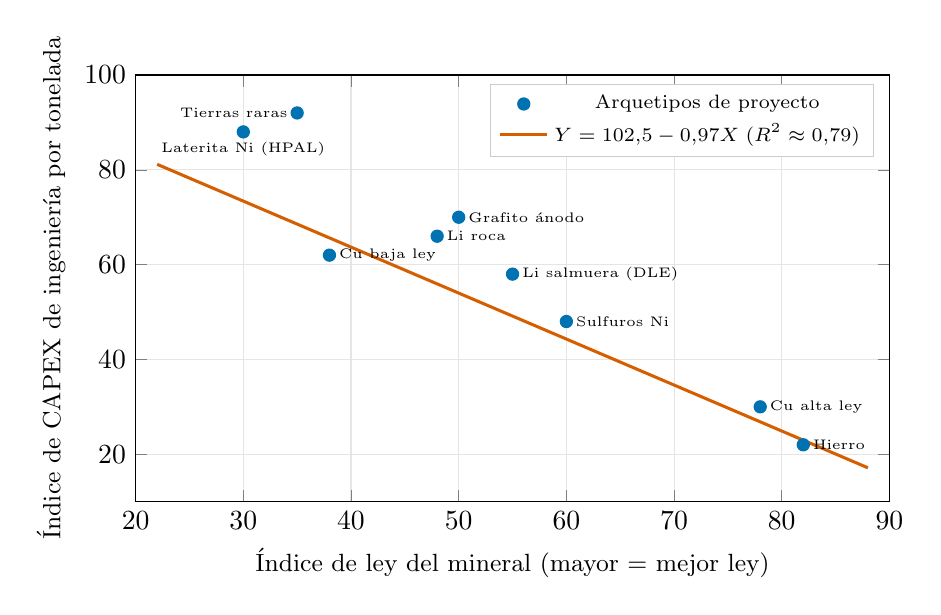
\begin{tikzpicture}
\begin{axis}[
  width=0.92\textwidth,height=7cm,
  xlabel={Índice de ley del mineral (mayor $=$ mejor ley)},
  ylabel={Índice de CAPEX de ingeniería por tonelada},
  xlabel style={font=\small},ylabel style={font=\small},
  xmin=20,xmax=90,ymin=10,ymax=100,
  ymajorgrids,xmajorgrids,grid style={gray!20},
  legend style={font=\scriptsize,at={(0.98,0.98)},anchor=north east,draw=gray!40}]
% Puntos
\addplot[only marks,mark=*,mark size=2.2pt,accentblue] coordinates
  {(78,30)(38,62)(60,48)(30,88)(55,58)(48,66)(50,70)(35,92)(82,22)};
\addlegendentry{Arquetipos de proyecto}
% Recta de regresión
\addplot[accentred,line width=1.1pt,domain=22:88,samples=2] {102.5-0.97*x};
\addlegendentry{$Y=102{,}5-0{,}97X\;(R^2\approx0{,}79)$}
% Etiquetas
\node[font=\tiny,anchor=west] at (axis cs:78,30) {Cu alta ley};
\node[font=\tiny,anchor=west] at (axis cs:82,22) {Hierro};
\node[font=\tiny,anchor=west] at (axis cs:38,62) {Cu baja ley};
\node[font=\tiny,anchor=west] at (axis cs:60,48) {Sulfuros Ni};
\node[font=\tiny,anchor=north] at (axis cs:30,88) {Laterita Ni (HPAL)};
\node[font=\tiny,anchor=west] at (axis cs:55,58) {Li salmuera (DLE)};
\node[font=\tiny,anchor=west] at (axis cs:48,66) {Li roca};
\node[font=\tiny,anchor=west] at (axis cs:50,70) {Grafito ánodo};
\node[font=\tiny,anchor=east] at (axis cs:35,92) {Tierras raras};
\end{axis}
\end{tikzpicture}
\caption[Dispersión ley de mineral vs.\ CAPEX de ingeniería]{Dispersión y correlación entre la ley del mineral y el CAPEX de
ingeniería por tonelada. La pendiente $\approx -1$ implica que cada caída de $\sim$10 puntos de ley añade $\sim$10 puntos de CAPEX
de ingeniería por tonelada. Los procesos novedosos (HPAL, separación de TR, purificación de grafito, DLE) se ubican en el
cuadrante de baja ley / alto CAPEX, donde se concentra la oportunidad de \emph{fee}. Elaboración propia.}
\label{fig:scatter}
\end{figure}

%=============================================================================
\chapter{Síntesis Estratégica y Recomendaciones}
%=============================================================================

\section{Matriz de priorización (atractivo $\times$ capacidad de ganar)}
\begin{table}[htbp]
\centering
\caption{Priorización de iniciativas para REDCO.}
\label{tab:priorizacion}
\footnotesize
\renewcommand{\arraystretch}{1.25}
\begin{tabularx}{\textwidth}{@{}Xccc@{}}
\toprule
\rowcolor{tablehead}
\textcolor{white}{\textbf{Iniciativa}} & \textcolor{white}{\textbf{Atractivo}} &
\textcolor{white}{\textbf{Capacidad}} & \textcolor{white}{\textbf{Prioridad}}\\
\midrule
Optimización de cobre \emph{brownfield} (Chile) & Alto & Alta & \textbf{1 --- Núcleo}\\
\rowcolor{tablealt}Estudios de litio (Argentina/Chile) & Muy alto & Media-alta & \textbf{2 --- Crecer}\\
\emph{Permitting} \& ESG \emph{engineering} & Muy alto & Media (a construir) & \textbf{3 --- Construir}\\
\rowcolor{tablealt}Ingeniería de níquel/grafito (Brasil/Canadá) & Alto & Media & \textbf{4 --- Selectivo}\\
EPCM \emph{greenfield} de gran escala & Medio (procíclico) & Media & \textbf{5 --- Oportunista}\\
\rowcolor{tablealt}Rusia / activos sancionados & n/a & n/a & \textbf{No-go}\\
\bottomrule
\end{tabularx}
\end{table}

\section{Hoja de ruta 2026--2030}
\begin{figure}[htbp]
\centering
\resizebox{0.96\textwidth}{!}{%
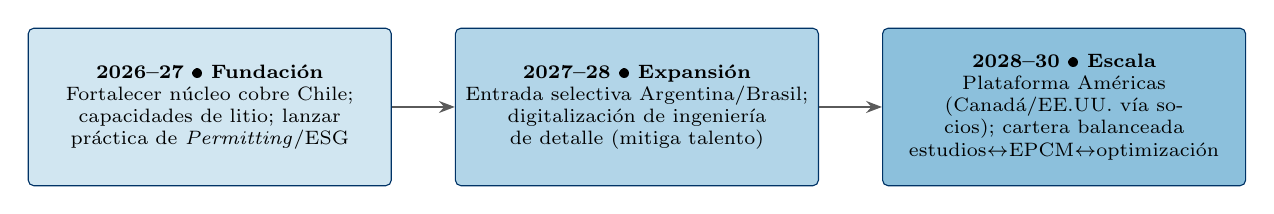
\begin{tikzpicture}[node distance=8mm]
  \node[flowbox,fill=accentblue!18,minimum width=4.6cm,minimum height=2cm,text width=4.4cm] (f1)
    {\textbf{2026--27 \textbullet{} Fundación}\\Fortalecer núcleo cobre Chile; capacidades de litio; lanzar práctica de \emph{Permitting}/ESG};
  \node[flowbox,fill=accentblue!30,minimum width=4.6cm,minimum height=2cm,text width=4.4cm,right=of f1] (f2)
    {\textbf{2027--28 \textbullet{} Expansión}\\Entrada selectiva Argentina/Brasil; digitalización de ingeniería de detalle (mitiga talento)};
  \node[flowbox,fill=accentblue!45,minimum width=4.6cm,minimum height=2cm,text width=4.4cm,right=of f2] (f3)
    {\textbf{2028--30 \textbullet{} Escala}\\Plataforma Américas (Canadá/EE.UU.\ vía socios); cartera balanceada estudios$\leftrightarrow$EPCM$\leftrightarrow$optimización};
  \draw[fl,line width=1pt] (f1) -- (f2);
  \draw[fl,line width=1pt] (f2) -- (f3);
\end{tikzpicture}}
\caption[Hoja de ruta estratégica 2026--2030]{Hoja de ruta de tres fases para la firma de ingeniería. Elaboración propia.}
\label{fig:roadmap}
\end{figure}

\section{Recomendaciones finales}
\begin{cajarecom}[Agenda estratégica para REDCO]
\begin{enumerate}[label=\textbf{\arabic*.}]
\item Concentrar el núcleo en \textbf{cobre + litio en el corredor de las Américas}; tratar Rusia como \emph{no-go} y Europa del
  Este solo vía \emph{joint venture}.
\item Construir las prácticas de \textbf{\emph{Permitting}/ESG y de Optimización}: los dos segmentos de mayor margen y crecimiento,
  y los que defienden los ingresos en la baja del ciclo.
\item \textbf{Industrializar la ingeniería de detalle} (\emph{digital twins}, automatización) para neutralizar el riesgo R3
  (talento) y proteger el margen.
\item \textbf{Gobernar la cartera por $\phi_{exec}$, no por precio}: la métrica de gestión debe ser la conversión de \emph{pipeline}
  a ingeniería facturada.
\item \textbf{Cubrir el CAPEX} con una combinación contractual y diversificación por mineral/país/cliente, para amortiguar el
  escenario pesimista.
\end{enumerate}
\end{cajarecom}

%=============================================================================
\appendix
\chapter{Metodología, Variables y Fuentes}
\label{ap:metodo}
%=============================================================================
\textbf{Enfoque.} Modelo \emph{top-down} de demanda de minerales $\rightarrow$ CAPEX inducido $\rightarrow$ \emph{fee pool} de
servicios, validado con \emph{benchmarks} \emph{bottom-up} de la fracción de ingeniería sobre CAPEX. Los escenarios se construyen
variando la CAGR de servicios, el factor de ejecución y la fracción de ingeniería (Ecuaciones~\ref{eq:vsvc}--\ref{eq:escenarios}).

\begin{table}[htbp]
\centering
\caption{Variables principales del modelo.}
\label{tab:variables}
\footnotesize
\renewcommand{\arraystretch}{1.25}
\begin{tabularx}{\textwidth}{@{}clX@{}}
\toprule
\rowcolor{tablehead}\textcolor{white}{\textbf{Símbolo}} & \textcolor{white}{\textbf{Definición}} & \textcolor{white}{\textbf{Rango usado}}\\
\midrule
$D_{m,t}$ & Demanda del mineral $m$ en el año $t$ & véase Tabla~\ref{tab:demanda-maestra}\\
\rowcolor{tablealt}$g_m$ & CAGR de demanda del mineral & 0{,}7\,\%--17\,\%\\
$\kappa_m$ & Intensidad de capital (USD/t de capacidad) & específico por mineral\\
\rowcolor{tablealt}$\theta_{eng}$ & Fracción de ingeniería sobre CAPEX & 0{,}04--0{,}07\\
$\theta_{op}$ & Fracción de consultoría sobre OPEX intervenido & 0{,}005--0{,}02\\
\rowcolor{tablealt}$\phi_{exec}$ & Factor de conversión \emph{pipeline}$\rightarrow$ingeniería & 0{,}70--0{,}95\\
$\beta$ & Elasticidad CAPEX--ley & $>0$\\
\bottomrule
\end{tabularx}
\end{table}

\textbf{Limitaciones.} Las cifras de demanda y de \emph{fee pool} son estimaciones trianguladas con incertidumbre material
($\pm$15--25\,\%). Las trayectorias suponen ausencia de \emph{shocks} macro extremos no contemplados en el escenario pesimista. La
asignación geográfica de CAPEX es indicativa.

\section{Registro de verificación (junio 2026)}
La Tabla~\ref{tab:verif} documenta la comparación entre el borrador inicial (cifras de memoria del analista) y la verificación con
fuentes públicas, indicando qué cambió y qué no se pudo confirmar.

\begin{table}[htbp]
\centering
\caption{Registro de verificación de cifras contra fuentes oficiales.}
\label{tab:verif}
\scriptsize
\renewcommand{\arraystretch}{1.25}
\resizebox{\textwidth}{!}{%
\begin{tabular}{@{}lllp{4.6cm}@{}}
\toprule
\rowcolor{tablehead}
\textcolor{white}{\textbf{Ítem}} & \textcolor{white}{\textbf{Verificado / ajustado}} &
\textcolor{white}{\textbf{Estado}} & \textcolor{white}{\textbf{Fuente principal}}\\
\midrule
Cobre 2024/2030 & 27 / 30 Mt (CAGR $\sim$1{,}8\,\%) & ajustado & IEA \emph{Copper}; S\&P Global~\cite{iea_gcmo2025,sp_copper}\\
\rowcolor{tablealt}Litio 2024/2030 & 1{,}0 / 2{,}6 Mt LCE & confirmado & Benchmark; Fastmarkets~\cite{benchmark_li,fastmarkets_li}\\
Cobalto 2030 & 0{,}27 Mt (ajuste a la baja) & ajustado & Cobalt Institute; IEA~\cite{iea_gcmo2025}\\
\rowcolor{tablealt}Níquel 2030 & 4{,}3 Mt & ajustado & Benchmark~\cite{benchmark_li}\\
Neodimio 2030 & 73 kt (imanes REE $+\sim\!\tfrac13$) & ajustado & IEA \emph{Rare Earths}~\cite{iea_gcmo2025}\\
\rowcolor{tablealt}Grafito 2024/2030 & 5{,}5 / 8{,}5 Mt & ajustado & IEA; USGS~\cite{iea_gcmo2025,usgs_mcs2025}\\
Silicio/polisilicio & 5{,}5 / 8{,}5 Mt & confirmado & IEA \emph{Solar PV}~\cite{iea_solar}\\
\rowcolor{tablealt}Plata 2030 & 44 kt (PV $\sim$10--14 kt/a) & confirmado & The Silver Institute~\cite{silver2025}\\
Aluminio total & 101 / 120 Mt ($+40\,\%$ vs.\ 2020) & reclasificado & International Aluminium Institute~\cite{iai_demand}\\
\rowcolor{tablealt}Acero 2030 & 1\,957 Mt ($+0{,}7\,\%$/a) & ajustado & OECD \emph{Steel Outlook 2025}~\cite{oecd_steel2025}\\
Mercado servicios & USD 14$\rightarrow$22 mil M (construido) & no verificable & EPCM global $\sim$USD 5{,}4 mil M~\cite{epcm_market}\\
\bottomrule
\end{tabular}}
\end{table}

\begin{cajanota}[Conclusión de la verificación]
La estructura del informe y los órdenes de magnitud se sostienen. Los ajustes principales fueron a la baja en cobalto, níquel y
neodimio (el borrador era optimista en \emph{battery/magnet minerals}) y una reclasificación del aluminio (total vs.\ primario). La
única cifra que no admite verificación a fuente única es el tamaño del mercado de servicios, que permanece como estimación
construida y declarada como tal.
\end{cajanota}

%=============================================================================
\chapter{Tablas de Datos Detalladas}
%=============================================================================
\section{Demanda por mineral y escenario (2030)}
\begin{table}[htbp]
\centering
\caption{Demanda por mineral y escenario al 2030.}
\label{tab:demanda-escenario}
\footnotesize
\renewcommand{\arraystretch}{1.25}
\resizebox{\textwidth}{!}{%
\begin{tabular}{@{}llrrrl@{}}
\toprule
\rowcolor{tablehead}
\textcolor{white}{\textbf{Mineral}} & \textcolor{white}{\textbf{Unidad}} &
\textcolor{white}{\textbf{Pesim.}} & \textcolor{white}{\textbf{Base}} & \textcolor{white}{\textbf{Optim.}} &
\textcolor{white}{\textbf{Referencia}}\\
\midrule
Litio & Mt LCE & 2{,}4 & 2{,}6 & 3{,}7 & Benchmark 2{,}4 $\cdot$ Albemarle 3{,}7~\cite{benchmark_li}\\
\rowcolor{tablealt}Cobalto & Mt & 0{,}24 & 0{,}27 & 0{,}31 & Cobalt Institute / IEA\\
Grafito & Mt & 7{,}0 & 8{,}5 & 11{,}0 & IEA; $\sim$11 Mt total a 2034\\
\rowcolor{tablealt}Níquel & Mt & 4{,}0 & 4{,}3 & 4{,}8 & Benchmark (batería $\sim$1{,}5 Mt)\\
Neodimio (imán) & kt & 68 & 73 & 85 & IEA: imanes REE $+\sim\!\tfrac13$\\
\rowcolor{tablealt}Silicio & Mt & 7{,}2 & 8{,}5 & 9{,}8 & IEA Solar PV~\cite{iea_solar}\\
Cobre & Mt & 29{,}0 & 30{,}0 & 31{,}5 & IEA STEPS~\cite{iea_gcmo2025}\\
\rowcolor{tablealt}Plata & kt & 41 & 44 & 50 & The Silver Institute~\cite{silver2025}\\
Aluminio (total) & Mt & 114 & 120 & 125 & IAI $+40\,\%$ a 2030~\cite{iai_demand}\\
\rowcolor{tablealt}Acero & Mt & 1\,930 & 1\,957 & 2\,100 & OECD~\cite{oecd_steel2025}\\
\bottomrule
\end{tabular}}
\end{table}

\section{Matriz numérica de los radares (siete geografías)}
\begin{table}[htbp]
\centering
\caption{Perfil de entorno / riesgo sistémico, escala 1--5 ($5=$ más favorable).}
\label{tab:radar-riesgo}
\scriptsize
\renewcommand{\arraystretch}{1.2}
\resizebox{\textwidth}{!}{%
\begin{tabular}{@{}lcccccc@{}}
\toprule
\rowcolor{tablehead}
\textcolor{white}{\textbf{Mercado}} & \textcolor{white}{Estab.\ pol.} & \textcolor{white}{Permisol.} &
\textcolor{white}{Geología} & \textcolor{white}{Costos} & \textcolor{white}{Talento} & \textcolor{white}{CAPEX/FX}\\
\midrule
Chile & 4{,}2 & 2{,}6 & 4{,}8 & 3{,}0 & 3{,}4 & 3{,}6\\
\rowcolor{tablealt}Brasil & 3{,}4 & 3{,}0 & 4{,}4 & 3{,}6 & 3{,}2 & 3{,}0\\
Argentina & 2{,}6 & 3{,}2 & 4{,}6 & 3{,}8 & 2{,}8 & 1{,}8\\
\rowcolor{tablealt}Canadá & 4{,}8 & 2{,}2 & 4{,}5 & 2{,}6 & 3{,}8 & 4{,}4\\
Europa Este & 3{,}0 & 2{,}8 & 3{,}2 & 3{,}4 & 3{,}0 & 3{,}0\\
\rowcolor{tablealt}Rusia & 1{,}6 & 2{,}4 & 4{,}7 & 4{,}0 & 2{,}6 & 1{,}4\\
EE.UU. & 4{,}0 & 2{,}0 & 4{,}0 & 2{,}4 & 3{,}6 & 4{,}2\\
\bottomrule
\end{tabular}}
\end{table}

\begin{table}[htbp]
\centering
\caption{Madurez de la demanda de ingeniería, escala 1--5 ($5=$ mayor tracción).}
\label{tab:radar-madurez}
\scriptsize
\renewcommand{\arraystretch}{1.2}
\resizebox{\textwidth}{!}{%
\begin{tabular}{@{}lcccccc@{}}
\toprule
\rowcolor{tablehead}
\textcolor{white}{\textbf{Mercado}} & \textcolor{white}{Pipeline} & \textcolor{white}{EPCM} &
\textcolor{white}{Optim.} & \textcolor{white}{Min.\ crít.} & \textcolor{white}{Madurez loc.} & \textcolor{white}{Apertura}\\
\midrule
Chile & 4{,}6 & 4{,}4 & 4{,}7 & 4{,}2 & 4{,}5 & 3{,}8\\
\rowcolor{tablealt}Brasil & 4{,}0 & 3{,}8 & 3{,}6 & 3{,}8 & 3{,}6 & 3{,}4\\
Argentina & 4{,}2 & 3{,}4 & 3{,}0 & 4{,}6 & 2{,}8 & 4{,}2\\
\rowcolor{tablealt}Canadá & 4{,}0 & 4{,}2 & 4{,}0 & 4{,}4 & 4{,}3 & 3{,}6\\
Europa Este & 3{,}4 & 3{,}0 & 3{,}2 & 3{,}6 & 2{,}8 & 4{,}0\\
\rowcolor{tablealt}Rusia & 2{,}6 & 3{,}4 & 3{,}6 & 3{,}2 & 3{,}2 & 1{,}4\\
EE.UU. & 4{,}4 & 4{,}5 & 4{,}4 & 4{,}5 & 4{,}4 & 3{,}0\\
\bottomrule
\end{tabular}}
\end{table}

\section{Valor del mercado de servicios por región (2030, base)}
\begin{table}[htbp]
\centering
\caption{Distribución regional indicativa del \emph{fee pool} (2030, escenario base).}
\label{tab:region}
\footnotesize
\renewcommand{\arraystretch}{1.25}
\begin{tabularx}{\textwidth}{@{}Xccc@{}}
\toprule
\rowcolor{tablehead}
\textcolor{white}{\textbf{Región}} & \textcolor{white}{\textbf{Valor (USD mil M)}} &
\textcolor{white}{\textbf{Participación}} & \textcolor{white}{\textbf{CAGR 24--30}}\\
\midrule
Sudamérica (Chile, Argentina, Brasil) & 8{,}4 & 38\,\% & $\sim$9\,\%\\
\rowcolor{tablealt}Norteamérica (Canadá, EE.UU.) & 6{,}6 & 30\,\% & $\sim$10\,\%\\
Resto del mundo (OCDE/aliados) & 4{,}4 & 20\,\% & $\sim$7\,\%\\
\rowcolor{tablealt}Europa del Este & 1{,}5 & 7\,\% & $\sim$8\,\%\\
Otros & 1{,}3 & 5\,\% & $\sim$5\,\%\\
\midrule
\textbf{Total} & \textbf{22{,}2} & \textbf{100\,\%} & \textbf{$\sim$8\,\%}\\
\bottomrule
\end{tabularx}
\end{table}

%=============================================================================
\chapter*{Referencias}
\addcontentsline{toc}{chapter}{Referencias}
%=============================================================================
\begin{thebibliography}{99}
\footnotesize
\bibitem{iea_gcmo2025} International Energy Agency (IEA). \textit{Global Critical Minerals Outlook 2025}. París, 2025.
  \url{https://www.iea.org/reports/global-critical-minerals-outlook-2025}.
\bibitem{usgs_mcs2025} U.S.\ Geological Survey (USGS). \textit{Mineral Commodity Summaries 2025}. Reston, VA, 2025.
  \url{https://pubs.usgs.gov/periodicals/mcs2025/mcs2025.pdf}.
\bibitem{oecd_steel2025} OECD. \textit{OECD Steel Outlook 2025}. OECD Publishing, París, 2025.
  \url{https://www.oecd.org/en/publications/oecd-steel-outlook-2025_28b61a5e-en.html}.
\bibitem{iai_demand} International Aluminium Institute (IAI). \textit{Global aluminium demand to reach new highs}
  (demanda $+40\,\%$ a 2030: 86{,}2 $\rightarrow$ 119{,}5 Mt). Londres, 2022--2025.
  \url{https://international-aluminium.org/}.
\bibitem{silver2025} The Silver Institute \& Metals Focus. \textit{World Silver Survey 2025}. Washington D.C., 2025.
  \url{https://www.silverinstitute.org/}.
\bibitem{benchmark_li} Benchmark Mineral Intelligence. \textit{Lithium / Nickel Forecasts} y
  \textit{Lithium industry needs over USD~116 billion to meet 2030 targets}. 2024--2025.
  \url{https://www.benchmarkminerals.com/}.
\bibitem{fastmarkets_li} Fastmarkets. \textit{Lithium supply and demand to 2030}. 2024.
  \url{https://www.fastmarkets.com/insights/lithium-supply-and-demand-to-2030/}.
\bibitem{iea_solar} International Energy Agency (IEA). \textit{Solar PV Global Supply Chains}. París, 2022.
  \url{https://www.iea.org/reports/solar-pv-global-supply-chains}.
\bibitem{sp_copper} S\&P Global Commodity Insights. \textit{The Future of Copper: Will the looming supply gap short-circuit
  the energy transition?} 2022. \url{https://www.spglobal.com/}.
\bibitem{epcm_market} Business Research Insights / Global Growth Insights. \textit{Engineering, Procurement \& Construction
  Management (EPCM) Market Report} (mercado global $\sim$USD~5{,}4 mil M en 2025; CAGR $\sim$8{,}4\,\%; segmento minero
  $\sim$USD~1{,}2 mil M). 2025. \url{https://www.businessresearchinsights.com/}.
\bibitem{bnef} BloombergNEF. \textit{Transition Metals Outlook} y \textit{Electric Vehicle Outlook}. 2024--2025.
\bibitem{woodmac} Wood Mackenzie. \textit{Global mining capital expenditure and metals demand outlooks}. 2024--2025.
\end{thebibliography}

\vfill
{\footnotesize\color{darkgray}\textit{Documento generado siguiendo la metodología de la \emph{skill} \texttt{market-research-reports},
adaptada a un reporte íntegramente en \LaTeX{} con toda la diagramación construida en TikZ/pgfplots. Las cifras de demanda de
minerales provienen de fuentes oficiales verificadas; el valor del mercado de servicios es una estimación construida del analista,
no un dato auditado.}\par}

\end{document}
